%%%%%%%%%%%%%%%%%%%%%%%%%%%%%%%%%%%%%%%%%
% Masters/Doctoral Thesis 
% LaTeX Template
% Version 2.5 (27/8/17)
%
% This template was downloaded from:
% http://www.LaTeXTemplates.com
%
% Version 2.x major modifications by:
% Vel (vel@latextemplates.com)
%
% This template is based on a template by:
% Steve Gunn (http://users.ecs.soton.ac.uk/srg/softwaretools/document/templates/)
% Sunil Patel (http://www.sunilpatel.co.uk/thesis-template/)
%
% Template license:
% CC BY-NC-SA 3.0 (http://creativecommons.org/licenses/by-nc-sa/3.0/)
%
%%%%%%%%%%%%%%%%%%%%%%%%%%%%%%%%%%%%%%%%%

%----------------------------------------------------------------------------------------
%	PACKAGES AND OTHER DOCUMENT CONFIGURATIONS
%----------------------------------------------------------------------------------------

\documentclass[
12pt, % The default document font size, options: 10pt, 11pt, 12pt
oneside, % Two side (alternating margins) for binding by default, uncomment to switch to one side
english, % ngerman for German
onehalfspacing, %singlespacing, % Single line spacing, alternatives: onehalfspacing or doublespacing
%draft, % Uncomment to enable draft mode (no pictures, no links, overfull hboxes indicated)
%nolistspacing, % If the document is onehalfspacing or doublespacing, uncomment this to set spacing in lists to single
%liststotoc, % Uncomment to add the list of figures/tables/etc to the table of contents
%toctotoc, % Uncomment to add the main table of contents to the table of contents
%parskip, % Uncomment to add space between paragraphs
%nohyperref, % Uncomment to not load the hyperref package
headsepline, % Uncomment to get a line under the header
%chapterinoneline, % Uncomment to place the chapter title next to the number on one line
%consistentlayout, % Uncomment to change the layout of the declaration, abstract and acknowledgements pages to match the default layout
]{Structural} % The class file specifying the document structure
\setcounter{secnumdepth}{4} %numbering 

\usepackage[toc,page]{appendix}

\usepackage[utf8]{inputenc} % Required for inputting international characters
\usepackage[T1]{fontenc} % Output font encoding for international characters
\usepackage{physics} %for physics simbols as kets 
\usepackage{mathpazo} % Use the Palatino font by default
\usepackage{float}
%\usepackage[backend=bibtex,style=authoryear,natbib=true]{biblatex} % Use the bibtex backend with the authoryear citation style (which resembles APA)
%\usepackage{biblatex} 
%\bibliography{Bibliography}%referencias
%\addbibresource{Bibliography.bib} % The filename of the bibliography
\usepackage[nottoc,notlot,notlof]{tocbibind}
\usepackage[autostyle=true]{csquotes} % Required to generate language-dependent quotes in the bibliography

%----------------------------------------------------------------------------------------
%	MARGIN SETTINGS
%----------------------------------------------------------------------------------------

\geometry{
	paper=a4paper, % Change to letterpaper for US letter
	inner=2.5cm, % Inner margin
	outer=3.8cm, % Outer margin
	bindingoffset=.5cm, % Binding offset
	top=1.5cm, % Top margin
	bottom=1.5cm, % Bottom margin
	%showframe, % Uncomment to show how the type block is set on the page
}

%----------------------------------------------------------------------------------------
%	THESIS INFORMATION
%----------------------------------------------------------------------------------------

\thesistitle{Two-Photon Imaging Using Tunable Spatial Correlations} % Your thesis title, this is used in the title and abstract, print it elsewhere with \ttitle
\supervisor{Dr. Alejandra \textsc{Valencia}} % Your supervisor's name, this is used in the title page, print it elsewhere with \supname
%\supervisor{Dr. Mayerlin}
\examiner{} % Your examiner's name, this is not currently used anywhere in the template, print it elsewhere with \examname
\degree{Physicist} % Your degree name, this is used in the title page and abstract, print it elsewhere with \degreename
\author{Juan \textsc{Vargas}} % Your name, this is used in the title page and abstract, print it elsewhere with \authorname
\addresses{} % Your address, this is not currently used anywhere in the template, print it elsewhere with \addressname

\subject{Physics Sciences} % Your subject area, this is not currently used anywhere in the template, print it elsewhere with \subjectname
\keywords{} % Keywords for your thesis, this is not currently used anywhere in the template, print it elsewhere with \keywordnames
\university{\href{https://uniandes.edu.co}{Universidad de Los Andes}} % Your university's name and URL, this is used in the title page and abstract, print it elsewhere with \univname
\department{\href{https://fisica.uniandes.edu.co/en/}{Physics Department}} % Your department's name and URL, this is used in the title page and abstract, print it elsewhere with \deptname
\group{\href{https://opticacuantica.uniandes.edu.co/index.php/en/home}{Quantum Optics}} % Your research group's name and URL, this is used in the title page, print it elsewhere with \groupname
\faculty{\href{https://ciencias.uniandes.edu.co}{Science Faculty}} % Your faculty's name and URL, this is used in the title page and abstract, print it elsewhere with \facname

\AtBeginDocument{
\hypersetup{pdftitle=\ttitle} % Set the PDF's title to your title
\hypersetup{pdfauthor=\authorname} % Set the PDF's author to your name
\hypersetup{pdfkeywords=\keywordnames} % Set the PDF's keywords to your keywords
}

\begin{document}

\frontmatter % Use roman page numbering style (i, ii, iii, iv...) for the pre-content pages

\pagestyle{plain} % Default to the plain heading style until the thesis style is called for the body content

%----------------------------------------------------------------------------------------
%	TITLE PAGE
%----------------------------------------------------------------------------------------

\begin{titlepage}
\begin{center}

\vspace*{.06\textheight}
{\scshape\LARGE \univname\par}\vspace{1.5cm} % University name
\textsc{\Large Thesis}\\[0.5cm] % Thesis type

\HRule \\[0.3cm] % Horizontal line
{\huge \bfseries \ttitle\par}\vspace{0.3cm} % Thesis title
\HRule \\[1.4cm] % Horizontal line
 
\begin{minipage}[t]{0.3\textwidth}
\begin{flushleft} \large
\emph{Author:}\\
{\authorname} % Author name - remove the \href bracket to remove the link
\end{flushleft}
\end{minipage}
\begin{minipage}[t]{0.3\textwidth}
\begin{flushright} \large
\emph{Supervisor:} \\
{\supname} % Supervisor name - remove the \href bracket to remove the link  
\end{flushright}
\end{minipage}\\[2cm]
 
%\vfill

\large \textit{A thesis submitted in fulfillment of the requirements\\ for the degree of \degreename}\\[0.3cm] % University requirement text
\textit{in the}\\[0.3cm]
\groupname\\\deptname\\[2cm] % Research group name and department name
 
%\vfill

\includegraphics[width=0.075\textwidth]{Logo.png} % University/department logo - uncomment to place it
 
{\large \today}\\[2.7cm] % Date

\vfill
\end{center}
\end{titlepage}

%----------------------------------------------------------------------------------------
%	DECLARATION PAGE
%----------------------------------------------------------------------------------------

\begin{declaration}
\addchaptertocentry{\authorshipname} % Add the declaration to the table of contents
\noindent I, \authorname, declare that this thesis titled, \enquote{\ttitle} and the work presented in it are my own. I confirm that:

\begin{itemize} 
\item This work was done wholly or mainly while in candidature for a research degree at this University.
\item Where any part of this thesis has previously been submitted for a degree or any other qualification at this University or any other institution, this has been clearly stated.
\item Where I have consulted the published work of others, this is always clearly attributed.
\item Where I have quoted from the work of others, the source is always given. With the exception of such quotations, this thesis is entirely my own work.
\item I have acknowledged all main sources of help.
\item Where the thesis is based on work done by myself jointly with others, I have made clear exactly what was done by others and what I have contributed myself.\\
\end{itemize}
 
\noindent Signed:\\
\rule[0.5em]{25em}{0.5pt} % This prints a line for the signature
 
\noindent Date:\\
\rule[0.5em]{25em}{0.5pt} % This prints a line to write the date
\end{declaration}

\cleardoublepage

%----------------------------------------------------------------------------------------
%	QUOTATION PAGE
%----------------------------------------------------------------------------------------

\vspace*{0.2\textheight}

\noindent\enquote{\itshape Nonesenses... later due}\bigbreak

\hfill N.N

%----------------------------------------------------------------------------------------
%	ABSTRACT PAGE
%----------------------------------------------------------------------------------------

\begin{abstract}
\addchaptertocentry{\abstractname} % Add the abstract to the table of contents
Two-Photon Imaging is a well studied fenomena, where we take advantage of the diferent correlations in wich the light can be related to recontruct the image of certain objects. In this Thesis use diferent spatial correlations of a SPDC light source, where we change this correlations changing the pump waist.
\end{abstract}

%----------------------------------------------------------------------------------------
%	ACKNOWLEDGEMENTS
%----------------------------------------------------------------------------------------

\begin{acknowledgements}
\addchaptertocentry{\acknowledgementname} % Add the acknowledgements to the table of contents
The acknowledgments and the people to thank go here, don't forget to include your project advisor\ldots
s 

\end{acknowledgements}

%----------------------------------------------------------------------------------------
%	LIST OF CONTENTS/FIGURES/TABLES PAGES
%----------------------------------------------------------------------------------------

\tableofcontents % Prints the main table of contents

\listoffigures % Prints the list of figures

%\listoftables % Prints the list of tables

%----------------------------------------------------------------------------------------
%	ABBREVIATIONS
%----------------------------------------------------------------------------------------

%\begin{abbreviations}{ll} % Include a list of abbreviations (a table of two columns)

%\textbf{LAH} & \textbf{L}ist \textbf{A}bbreviations \textbf{H}ere\\
%\textbf{WSF} & \textbf{W}hat (it) \textbf{S}tands \textbf{F}or\\

%\end{abbreviations}

%----------------------------------------------------------------------------------------
%	PHYSICAL CONSTANTS/OTHER DEFINITIONS
%----------------------------------------------------------------------------------------

%\begin{constants}{lr@{${}={}$}l} % The list of physical constants is a three column table

% The \SI{}{} command is provided by the siunitx package, see its documentation for instructions on how to use it

%Speed of Light & $c_{0}$ & \SI{2.99792458e8}{\meter\per\second} (exact)\\
%Constant Name & $Symbol$ & $Constant Value$ with units\\

%\end{constants}

%----------------------------------------------------------------------------------------
%	SYMBOLS
%----------------------------------------------------------------------------------------

%\begin{symbols}{lll} % Include a list of Symbols (a three column table)

%$a$ & distance & \si{\meter} \\
%$P$ & power & \si{\watt} (\si{\joule\per\second}) \\
%Symbol & Name & Unit \\

%\addlinespace % Gap to separate the Roman symbols from the Greek

%$\omega$ & angular frequency & \si{\radian} \\

%\end{symbols}

%----------------------------------------------------------------------------------------
%	DEDICATION
%----------------------------------------------------------------------------------------

\dedicatory{For/Dedicated to/To my\ldots} 

%----------------------------------------------------------------------------------------
%	THESIS CONTENT - CHAPTERS
%----------------------------------------------------------------------------------------

\mainmatter % Begin numeric (1,2,3...) page numbering

\pagestyle{thesis} % Return the page headers back to the "thesis" style

% Include the chapters of the thesis as separate files from the Chapters folder
% Uncomment the lines as you write the chapters

% Chapter Template

\chapter{Introduction} % Main chapter title

\label{Chapter1} % Change X to a consecutive number; for referencing this chapter elsewhere, use \ref{ChapterX}

%----------------------------------------------------------------------------------------
%	SECTION 1
%----------------------------------------------------------------------------------------

\section{Imaging}
Intensity \cite{physicsGhost}

%-----------------------------------
%	SUBSECTION 1
%-----------------------------------
\section{Two-Photon Imaging}

\subsection{Two-Photon Imaging using entangled photon pairs}
A two-photon optical imaging experiment was perfomed based on the quantum nature of the \textit{signal} and \textit{idler}
photons pairs produced in spontaneous parametric down-conversion\cite{pittman}.
\begin{figure}[h]
\centering
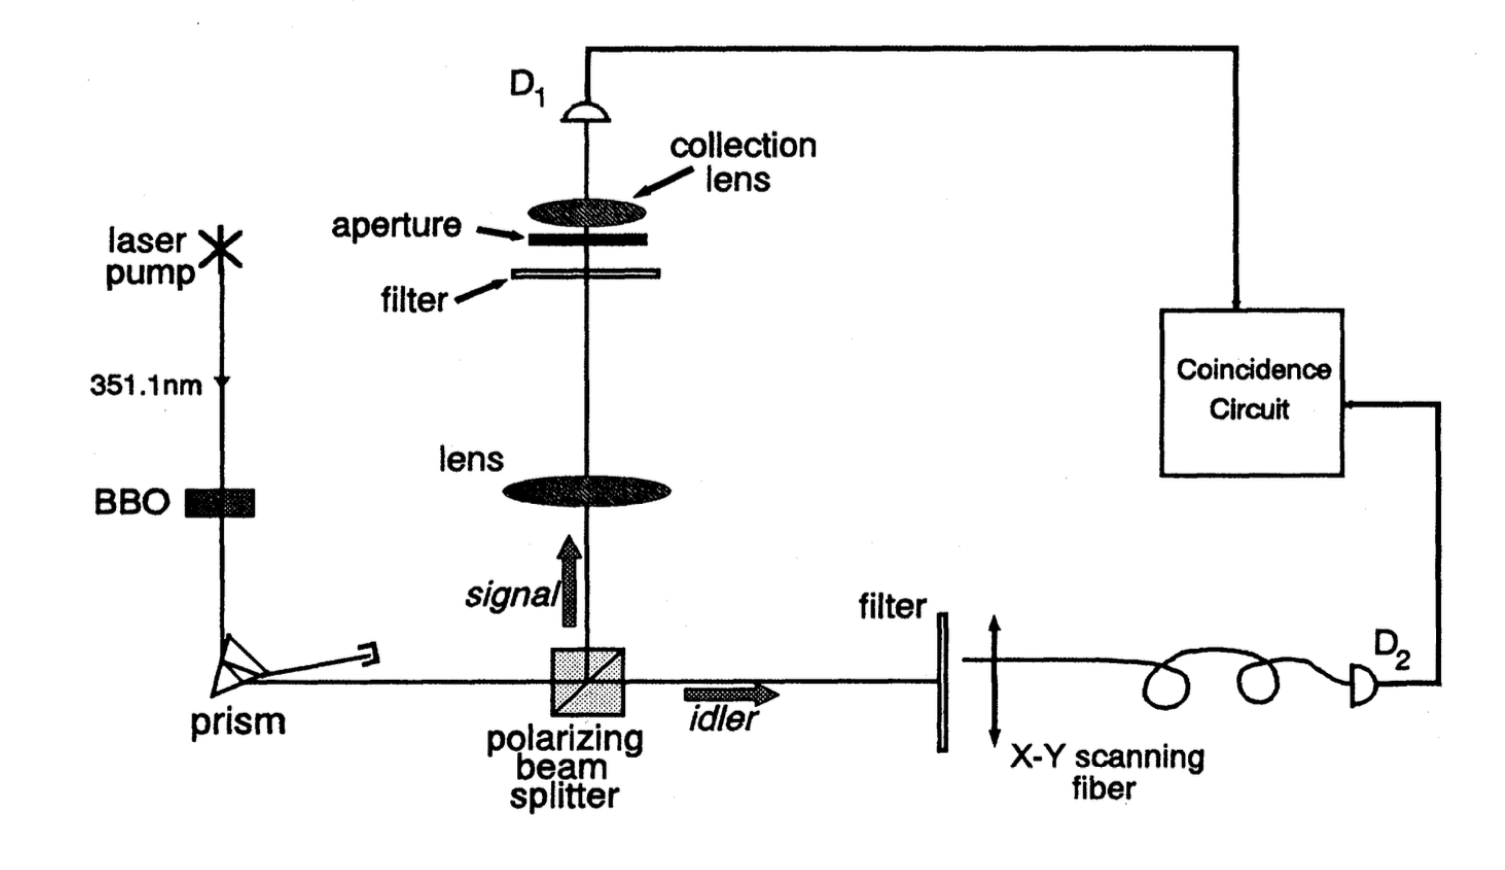
\includegraphics[width=0.5\textwidth]{Figures/pittman.png}
\caption{Cartoon schematic of the experimental setup used by Pittman, Taken from \cite{pittman}} 
\label{fig:pittman}
\end{figure}
An important fact of this experiment is the use of a lens in the signal beam that establishes an image plane with the definitive point-by-point correspondence object(mask) plane.




\subsection{Two-photon Imaging Using Thermal Sources}

In \cite{thermal} they compared ghost Imaging using entanglement versus Classical correlated light. read and information in \cite{thermalAlejandra}. here i talk about coherence and intensity fluctuations \cite{intensity}

\subsection{Simulations}

No\cite{simulated}
%----------------------------------------------------------------------------------------
%	SECTION 2
%----------------------------------------------------------------------------------------




% Chapter Template

\chapter{Theory} % Main chapter title

\label{Chapter2} % Change X to a consecutive number; for referencing this chapter elsewhere, use \ref{ChapterX}

In Here we will discus some important facts to get a complete understanding 
in the physical phenomena that is happening. Specially we will develop the 
notions that are crucial in the understanding of the Two-photon imaging using entangled light, been this said 
we will start talking about correlations.

\section{Correlations between two photons}

The term "correlation" is crucial at this point, and it refers to the relation of two or more situations have. For example 
we can establish a correlations between the US dolar currency exchange rate and the prices of technology in one country. These two things have direct relation, if one blows up, the other one will too.
These two situations, or variables, can have a strong correlations or a week one. \\

Indeed in quantum physics we can have a pair of photons that are so strongly correlated, in their possible variables (spatial and temporal),
that we say they are entangled. This statment can leads us 
to a dense discussion about the nature of this entanglement, 
a discussion that were started between Einstein and Bohr in the first years of quantum physics \cite{einstein}.\\

To avoid this discussion we will just talk about correlations, 
and when referring about a pair of correlated photons, we will mean that 
this pair of photons are correlated in one or varius of their variables. 
They can be correlated in momentum, meaning that when one photon have a given $\vec{q}_i$ momentum 
and the other photon have a $\vec{q}_j$ momentum that is determined by the first, this relations is the momentum correlations a we can work out an expression for this relationship.
\subsection{SPDC}

As the title of this work implies, we need a source light that produces pair of photons, 
and we would like to exploit the advantages of strong correlations between them.
The photons generated via spontaneous parametric down conversion (SPDC) are
widely used in quantum optics experiments. The popularity of this source of paired
photons is strongly related to the relative simplicity of its experimental
realisation, and to the variety of quantum features that down converted photons can exhibit. 
The generated photons via SPDC can be correlated in different degrees of freedom, for example 
in polarisation, in frequency and in the equivalent degrees of freedom: 
'orbital angular momentum, space and transverse momentum \cite{spatiocorrelations}.\\

\begin{figure}[h!]
\centering
\label{fig:spdcSimple}
 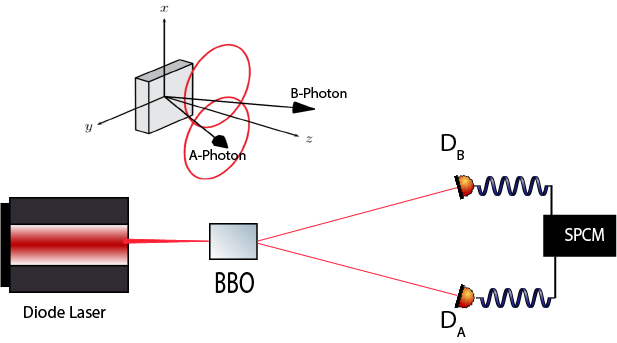
\includegraphics[width=0.65\textwidth]{Figures/spdcSimple.png}
 \caption{Simple Experimental setup for the type-II noncollinear SPDC process} 
\end{figure}


SPDC is an optical process in which focus a beam pump, that is 
propagating in the $z$-direction, to a nonlinear crystal of length $L$. Depending of the polarisation
direction of the produced photons, the nonlinear crystals can be classified in types. The type-0 crystal will 
produce pairs that are polarised in the source light direction. The type-I will do the proper, but this time the polarisation will be in the 
perpendicular direction of the pump. The last type, type-two crystal will produce a pair of photons, 
one with the polarisation in the sa,e direction as the pump, and the other one perpendicular. 
The generated pair can emerge from the crystal in a collinearly or noncollinearly.


Using first order perturbation 
and the paraxial approximation, the two-photon state is given by:
\begin{equation}
\label{eq:stateFunComplex}
\ket{\Psi}=\int dq_B dq_A d\Omega_B d\Omega_A 
\times [\Phi(q_B,\Omega_B;q_A,\Omega_A) \hat{a}^{\dagger} (\Omega_B,q_B) \hat{a}^{\dagger}(\Omega_A,q_A) \\
+ \Phi(q_A,\Omega_A;q_B,\Omega_B) \hat{a}^{\dagger}(\Omega_B,q_B) \hat{a}^{\dagger}(\Omega_A,q_A)]   \ket{0}  
\end{equation}
Where this state function depends on the transverse wave vectors $q_n=(q_n^x,q_n^y)$ and frequency detuning, $\Omega_n=\omega_n-\omega_0^n$, 
around the central frequencies, $\omega_0^n$, for the photon at the path $A$ or $B$ ($n=A,B$).
The $\Phi(q_B,\Omega_B;q_A,\Omega_A)$ and $\Phi(q_A,\Omega_A;q_B,\Omega_B)$
are the mode functions or biphotons that contains all the informations about the correlations
between the pair of down-converted photons. The operator $\hat{a}^{\dagger}$ indicates the creations of an $n$-polarized photon with transverse momentum $q_n$, 
and frequency detuning $\Omega_n$ \cite{physicsGhost}. \\

In the optical table we put a polariser at certain directions at the detections modules,
filtering some of the photons before reaching the detector, this filtering also have a mathematical effect in our model, 
it is posible now to write \ref{eq:stateFunComplex} different, dropping one term:
\begin{equation}
\label{eq:stateFun}
\ket{\Psi}=\int dq_B dq_A d\Omega_B d\Omega_A 
\times [\Phi(q_B,\Omega_B;q_A,\Omega_A) \hat{a}^{\dagger} (\Omega_B,q_B) \hat{a}^{\dagger}(\Omega_A,q_A) 
] \ket{0}  
\end{equation}

The mode function  $\Phi(q_B,\Omega_B;q_A,\Omega_A)$ is related with the joint probability of detecting both an $B$-polarized
photon, with tranverse momentum $q_B$ and frequency detuning $\Omega_B$, at the detector $B$ 
and an $A$-polarized
photon, with tranverse momentum $q_A$ and frequency detuning $\Omega_A$, at the detector $A$. 

\subsubsection{Phase matching conditions}
In particular, $\Phi(q_B,\Omega_B;q_A,\Omega_A)$ reads \cite{spatiocorrelations}:
\begin{equation}
\label{eq:mode}
\Phi(q_B,\Omega_B;q_A,\Omega_A) = \mathcal{N} \alpha(\Delta_0,\Delta_1) \beta(\Omega_B,\Omega_A) \times
sinc \left( \frac{\Delta_k L}{2} \right) e^{i \frac{\Delta_k L}{2}}
\end{equation}
Where $\mathcal{N}$ is a normalisation constant, $\alpha(\Delta_0,\Delta_1)$
and $\beta(\Omega_B,\Omega_A)$yields the informations of the pump's transverse 
and spectral distribution, respectively, L is the length of the nonlinear crystal.
For the process that is happening inside the crystal, there are some conditions that have to be fulfilled. These conditions are related with the energy and momentum conservations inside the parametric down conversion process.
The terms $\Delta_0$, $\Delta_1$ and $\Delta_k$ are functions that result from the phase matching conditions and read:
\begin{equation}
\Delta_0=q_B^x + q_A^x
\end{equation}
\begin{equation}
\Delta_1= q_A^y cos\phi_A + q_B^y cos\phi_B - N_B \Omega_B sin\phi_B + N_A \Omega_A sin\phi_A - \rho_B q_B^x sin\phi_B 
\end{equation}
\begin{equation}
\Delta_k=N_p(\Omega_B+\Omega_A)-N_B\Omega_B cos\phi_B - N_A\Omega_A cos\phi_A -q_B^y sin\Omega_B + q_A^y sin\Omega_A + \rho_p \Delta_0 - \rho_B q_B^x cos\phi_B
\end{equation}
The angles $\phi_B$ and $\phi_A$ are the creation angles of the down-
converted photons inside the crystal with respect to the pump’s
propagation direction, whereas the angles $\rho_p$ and $\rho_B$ account for
the walk-off of the pump $p$ and the $B$ down-
converted photon, respectively. 
In this study, $\phi_B$ and $\phi_A$ are treated as constants, 
mainly because the scanned transverse momentum regions represent a small portion around
the emission angles. $N_n$ denotes the inverse of the group velocity for each photon.



\subsection{Spatial Correlations}

In order to observe the correlations presented in \ref{eq:mode} we have to take into account some considerations about the descrption of the things we have in optical table.
First of all we have a pump beam with a Gaussian profile with waist $w_p$ 
in such way that $\alpha (\Delta_0,\Delta_1 ) \propto \text{exp}[-w_p^2 (\Delta_0^2 + \Delta_1^2 )/4]$, a CW pump laser, mathematically represented by
$\beta (\Omega_B , \Omega_A) \propto \delta(\Omega_B + \Omega_A)$. Making the aproximations for the sinc function by a Gaussian fuctions with the same width at $1/e^2$ of its maximum,
i.e., $sinc(x) \approx \text{exp}(-\gamma x^2)$ with $\gamma$ equal $0.193$.
The mode function reduces to:

\begin{equation}
\label{eq:modeSim}
\Phi(q_B,\Omega_B;q_A,\Omega_A) = \mathcal{N} \beta (\Omega_B , \Omega_A)
\times \textit{exp}\left[ -\frac{w_p^2 (\Delta_0^2 + \Delta_1^2 )}{4}-\gamma \left(\frac{\Delta_k L}{2} \right)^2 + i\frac{\Delta_k L}{2} \right]  
\end{equation}

In order to observe the transverse correlations (spatial correlations), the 
frequency information has to be traced out, in the optical table this can
be achieved by placing some interferometer filters before detection. This spectral
filters are modeled as $f_n (\Omega_n)=\text{exp}[-\Omega_n^2/(4\sigma_n^2)]$, with bandwidth $\sigma_n$ chosen to achive a regimen where the 
spatial-spectral correlations are completely broken \cite{broke}. 
To achieve this mathematically we have to integrate \ref{eq:modeSim} around the
spatial variables:
\begin{equation}
\label{eq:modeSpa}
\tilde{\Phi}(q_B,q_A) = \int d\Omega_B d\Omega_A f_B(\Omega_B)f_A(\Omega_A) \Phi(q_B,\Omega_B;q_A,\Omega_A)
\end{equation}

\begin{figure}[h!]
\centering
{  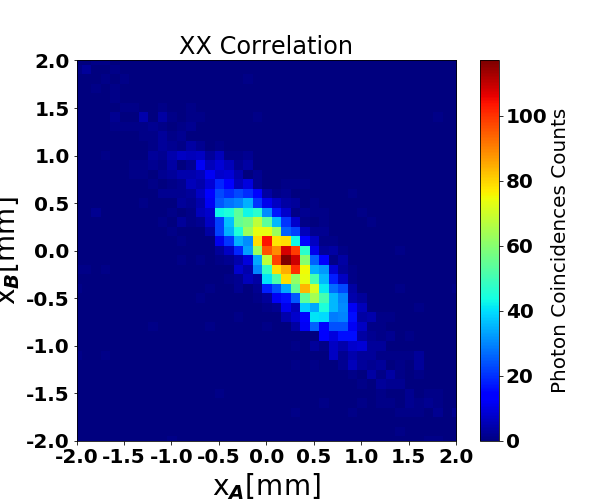
\includegraphics[width=0.48\textwidth]{Figures/xxCorrelation.png} }
{  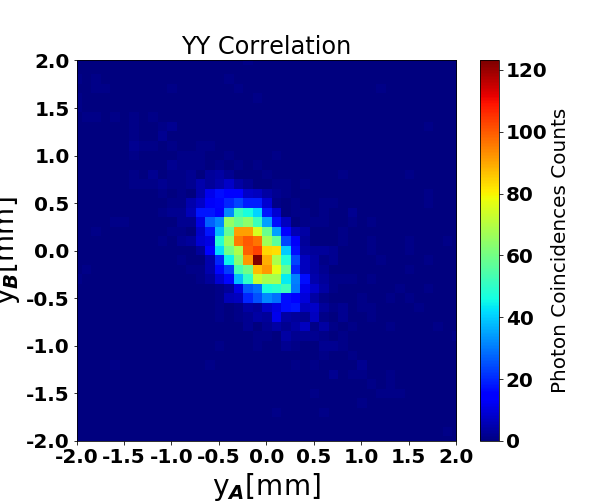
\includegraphics[width=0.48\textwidth]{Figures/yyCorrelation.png} }
\caption{Experimental Spatial correlations between a pair of down-converted photons. Right image shows the correlation in the x variable. Left shows the correlation in the y variable, Beam propagating in the z direction}
 \label{fig:corre}
\end{figure}
Figure \ref{fig:corre} show a couple of examples of how these correlations we are talking about look like. These correlations have some king of circular shape,
and show how strong is the posibility of detecting a photon at a given position, looking at the first graph, there is a great chance
of detecting simultaneously a photon at $x_B=0$ and at $x_A=0$. Now if we look at the left graph, it is showing the correlation 
of the pair of photons in the $y$ direction, there is a significant probability of measuring simultaneously a photon at $y_B=0.4$ 
and at $y_A=-0.4$. It is interesting how in this case there is a "negative" correlation, the expected position at which we will find the other photon, is at the same, but negative position.
Another interesting fact we have to point out, is that this correlations algo can be sharper, the x correlation have a more circular shape, making wider the posible values for a given $x_B$. In contrast the y correlation is more eliptic, meaning it restring the posible values por a given $y_B$.
It is easy to think how a strong correlation should look like, a strong correlations in spatial variables would mean that if we have the position of one photon at the position $x_B$ we immediately would know which $x_A$ have the other photon, this king of ideal spatial correlation would look like a straigth line
really thin, Figure \ref{fig:idealCorre}. 


\begin{figure}[h!]
\centering
{  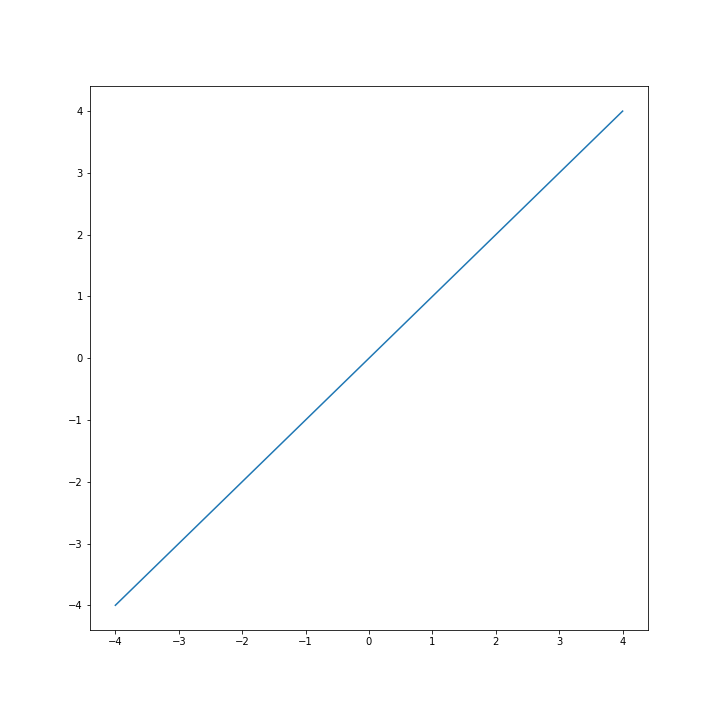
\includegraphics[width=0.48\textwidth]{Figures/idealPositiveCorrelation.png} }
{  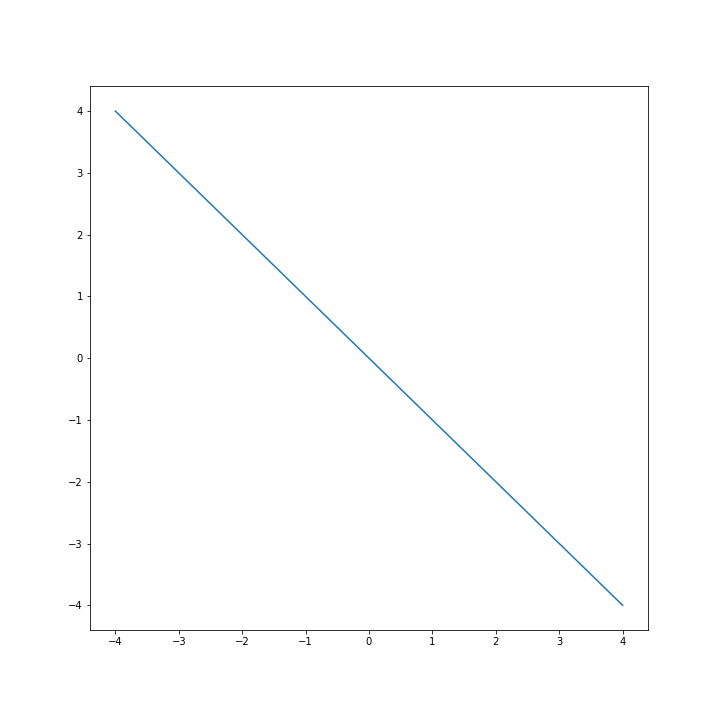
\includegraphics[width=0.48\textwidth]{Figures/idealNegativeCorrelation.png} }
\caption{Positive(right) and Negative(left) ideal spatial correlations}
 \label{fig:idealCorre}
\end{figure}

The Biphoton then takes a quadratic form\cite{spatiocorrelations}:
\begin{equation}
\label{eq:quadratic}
\tilde{\Phi}(q_B,q_A)=N exp\left[ -\frac{1}{2}x^T A x + i b^T x \right]
\end{equation}
where N is a normalization constant, that satisfies $\int \int | \tilde{\Phi}(q_B,q_A)|^2 d^2 q_B d^2 q_A = 1$. 
$x$ is a 4-dimensional vector defined as $x = (q^x_B, q^y_B ,q^x_A,q^y_A )$, $A$ 
is a 4 x 4 real-valued, symmetric, positive definite matrix and b is a 4- dimensional vector. 
A and b are defined from the phase-matching conditions of the SPDC process. $x^T$ and $b^T$ denote
 the transpose of $x$ and $b$. $A$ and $b$ are functions that depend of all the relevant 
parameters in the experiment such as the length of the crystal L, pump waist $w_p$, creation 
angles inside the crystal $\varphi_n$ and the width of the spectral filter $\sigma_n$.


To have a general numerical approach to $\tilde{\Phi}(\vec{q_B},\vec{q_A})$, it is desired to 
writte it as generic correlations instead of the experimental parameters. This can be done by 
noticing that the amplitude of $\tilde{\Phi}(\vec{q_B},\vec{q_A})$ has the form of a 4-dimensional 
gaussian distribution, given by
\begin{equation}
f(x) = \tilde{N}e^{-\frac{1}{2}x^T \Sigma^{-1}x},
\label{Gaussian}
\end{equation}
where  $\tilde{N}$ is a normalization constant satisfying $\int f(x) d^4 x = 1$, $\Sigma^{-1}$ is 
the inverse of the covariance matrix that contains the correlations between the different elements
 of $x$. With $x_i$ {$i=0,1,2,3$}, $\Sigma$ can be written as:
\begin{equation}
\Sigma_{ij} = \sigma_{x_i} \sigma_{x_j} \rho_{x_i x_j}
\label{eq:Pearson}
\end{equation}
where $\sigma_i$ denotes de square root of the variance of  $x_i$ and $\rho_{x_i x_j}$ denotes the 
Pearson correlation coefficient between $x_i$ and $x_j$. This coefficient quantifies how strong is 
the linear correlation between $x_i$ and $x_j$\cite{shafer}.
By using Eq.(\ref{eq:Pearson}), the correlations between the spatial variables of the photons 
can be manually modified in Eq.(\ref{eq:quadratic}).

STILL WORK TO DO!!! \\


A way to quantify the degree of spatial correlation we shall define 'correlation parameter':
\begin{equation}
K^\lambda = \frac{C^\lambda_{si}}{\sqrt{C^\lambda_{ss}C^\lambda_{ii}}}
\end{equation}
calculated for each direction $(\lambda = x, y)$ from the covariance matrix $C^\lambda$ with elements $C^\lambda_{kj} = \langle q^\lambda_k q^\lambda_j \rangle - \langle q^\lambda_k \rangle \langle q^\lambda_j \rangle $.



\subsection{Tunable Spatial Correlation SPDC source light}
It is clear that both \ref{eq:modeSim} and \ref{eq:modeSpa} depend on $w_p$, the pump waist. If we change this 
parameter and keep the rest of the parameters constant, the term in the exponential function $[-w_p^2 (\Delta_0^2 + \Delta_1^2 )/4]$ will variate,
making changes in the shape of the original mode function. As it was mentioned here before and in \cite{omar}, the mode function
contains all the informations about the correlations of the generated down converted photons. Hence changing the pump waist $w_p$
will change the correlations of the generated pair of photons.




\section{Imaging}

Assuming we have an object that have its own light or its externally illuminated,
imaging means collecting that light that is emitted from the object. Each point
of the surface of the object will emit spherical waves to all possible directions,
being this said, What is the probability to have a spherical wave collapsing into a point or small spot? 
Obviously, the chance is practically zero unless an imaging system is applied.
\\
The concept of optical imaging was well developed in classical optics and the Figure
\ref{fig:imaging} schematically illustrates a standar imaging setup. In this setup 
an object is illuminated by a radiation source, an imaging lens is used 
to focus the scattered and reflected light from the object onto an image plane 
which is defined by the “Gaussian thin lens equation”\cite{hecht}:
\begin{equation}
\frac{1}{S_o}+\frac{1}{S_i}=\frac{1}{f}
\end{equation}
 where $S_o$ is the distance between the object and the imaging lens, $S_i$ the distance 
between the imaging lens and the image plane, and $f$ the focal lenght of the imaging lens. This equation defines
a point-to-point relationship between the object plane and the image plane: any radiation starting from a point on the object will colapse at a certain point at the image plane.
\\
\begin{figure}[h!]
\centering
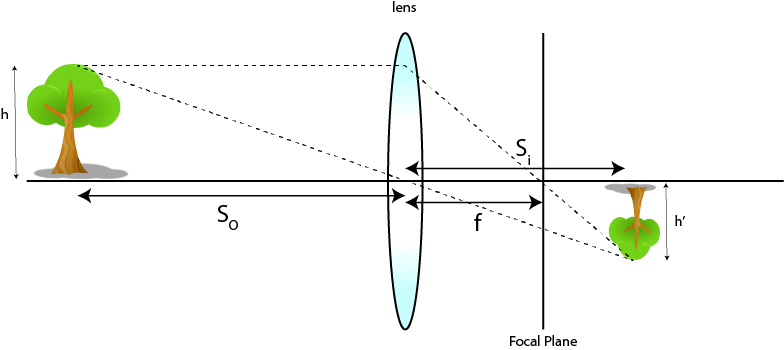
\includegraphics[width=0.6\textwidth]{Figures/imaging.png}
\caption{Optical imaging: a lens produces an image on an object at $S_i$. This distance is defined
by the Gaussian thin-lens equation} 
\label{fig:imaging}
\end{figure}
This one-to-one correspondence in the image-forming relationship between the object and the image planes produces a perfect image.
The observed image can be magnified or demagnified, for example, in the 
Figure \ref{fig:imaging} the original object is a tree, and it is demagnified at the image plane. This depends on which optical 
system are we using, what kind on lenses are involved and the distance between object and them.

\subsection{Standar Imaging}

The observed image is a reproduction of the illuminated object, mathematically
corresponding to a convolution between the object distribution fuction $ |T(\vec{\rho_o})|^2$ (aperture function) 
and a $\delta$-function, which is present for the perfect
point-to-point correspondence \cite{introquantumoptics}:
\begin{equation}
\label{eq:intensity}
\langle I(\vec{\rho_i}) \rangle =\int_{obj} d\vec{\rho_o} |T(\vec{\rho_o})|^2 \delta(\vec{\rho_o}+\frac{\vec{\rho_i}}{m})
\end{equation}
where $\langle I(\vec{\rho_i})\rangle $ is the mean intensity at the image plane, $\vec{\rho_o}$ and $\vec{\rho_i}$ are 2-D vectors of the
transverse coordinates, $\vec{\rho_n}= (x_n,y_n)$, in the object and image planes, respectively, and
$m=s_i/s_o$ is the image magnification factor.

In reality, we are limited by the finite size of the optical system, we may never obtain a perfect image.
The incomplete constructive-destructive interference turns the point-to-point correspondence into 
 a point-to-"spot" relationship. The $\delta$-function in the convolution of equation \ref{eq:intensity}
will be replaced by a point-to-"spot" image-forming function, or a point-spread function,
\begin{equation}
\label{eq:realIntensity}
\langle I(\vec{\rho_i}) \rangle =\int_{obj} d\vec{\rho_o} |T(\vec{\rho_o})|^2 \text{somb}^2[\frac{\pi D}{\lambda S_o} | \vec{\rho_o}+\frac{\vec{\rho_i}}{m}|]
\end{equation}

where the sombrero-like point-spread function is defined as 
somb$(x) \equiv  2J_1(x)/x$, with $J_1(x)$ the first-order Bessel function, and $D$ the diameter of the imaging lens.
It is clear from equation \ref{eq:realIntensity} that the finite size of the spot in the point-to-"spot" 
correspondence is determined by some parameters, if we want to have a almost-perfect correspondence we 
would like to not place the lens to far away from the object, $S_o$. A big imaging lens, and with "big" I refer to its diameter, $D$.
Imaging usually uses a wide variety of photons with deferents 
frequencies\footnote{Imaging forming, as the procces done by our eyes and brain uses a big range of
photon frequencies, this range is called the \textit{visible spectrum} ($\sim 390-700 nm$), the images produced by our eyes are formed just from photons 
that are at this frequencies, the rest of the photons are ignored by our eyes} 
if we were able to filter the light that illuminates the object, we would like to choose a short
wavelength $\lambda$. 

This finite size of the spot in the point-to-"spot" relationship we described before, is what is called 
spatial resolution. A higher spatial resolution of the image is achieved by the conditions described before. 
Another daily situation in which we are forming images, is when we take a picture. Cameras manufacteres play with this parameters
to achieve a high spatial resolution, a spot-to-pixel correspondence.
For further informations about this "real life" situation check the \ref{appendix:intensity}.



\subsection{Two-photon Imaging}\label{twoPhotonImaging}

Two-photon imaging consist after all, in reconstructing an image of an object. 
But in this case we use two dectector located in diferents paths of the light. 
By using the dectections of them separately we get a constant signal, with no information 
about the object, Figure \ref{fig:twoPhotonSetup}. But if instead we use the signal of them 
both, counting conincidences, we can reconstruct the double slit in 
Figure \ref{fig:twoPhotonSetup}. \\


\begin{figure}[h]
\centering
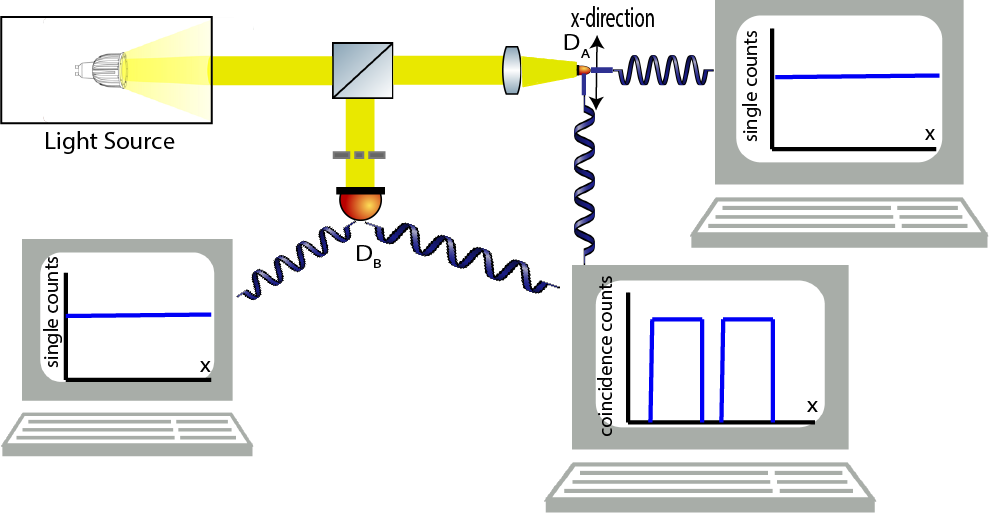
\includegraphics[width=0.75\textwidth]{Figures/twoPhotonSetup.png}
\caption{Simple schematic for the Two-photon Imaging} 
\label{fig:twoPhotonSetup}
\end{figure}

In order to reconstruct the image of the double slit, we have to introduce some kind of spatial 
dependence, the object, in this case the double slit, is distributed along a transverse direction 
of the light propagation. But what we have learnt is that scanning along the x-direction 
(asuming that light propagates along the z-direction), in the path that have no interaction 
with the object $D_A$, and colecting all the light that interacts with the object $D_B$, 
gathering no spatial information. We reconstruct the double slit in the coincidences counts, 
every time we have a photon detected going througt the double slit, and a photon at a certaint 
position $x_i$, we graph coincidences vs ${ x_i }$ and we get the image of the double slit, Figure \ref{fig:twoPhotonSetup}. 


The standar imaging used the photons at the image plane, to form the image. In other 
words it measures one photon per spot at the image plane. For the two-photon imaging, in certain 
aspects the behaviour is similar as that of the classical.
They both exhibit a similar point-to-point imaging-forming function, except the 
two-photon image is only reproducible in the joint-detection between two independent photodetectors,
and the point-to-point imaging-forming function is in the form of second-order correlation,
\begin{equation}\label{eq:coincidences}
R_{BA}(\vec{\rho_A})=\int_{obj} d\vec{\rho_B} |T(\vec{\rho_B})|^2 G^{(2)}(\vec{\rho_B},\vec{\rho_A})
\end{equation}
where $R_{BA}(\vec{\rho_B})$ is the joint-detection counting rate between photodetectors $D_B$ and $D_A$.
$G^{(2)}(\vec{\rho_B},\vec{\rho_A})$ is a nontrivial point-to-point second-order correlation
function, corresponding to the probability of observing a joint photo-detection event
at the coordinates $\vec{\rho_B}$ and $\vec{\rho_A}$. The physics behing $G^{(2)}(\vec{\rho_B},\vec{\rho_A})$
is what changes between the different kinds of two-photon imaging.

This second-order correlation functions is defined as\cite{introquantumoptics}:
\begin{equation}
G^{(2)} (\vec{\rho_B},\vec{\rho_A})= \frac{ \langle E^* (\vec{\rho_B}) E^* (\vec{\rho_A}) E^ (\vec{\rho_B}) E^ (\vec{\rho_A}) \rangle }{\langle |E^ (\vec{\rho_B})|^2 \rangle \langle |E^ (\vec{\rho_A})|^2 \rangle}
\end{equation}

%----------------------------------------------------------------------------------------
%	SECTION 1
%----------------------------------------------------------------------------------------
\subsubsection{Two-photon Imaging using entangled photon}

In the previous section we introduced the notion of two-photon imaging , but we didn't care 
much about the nature of the source light. For this case we will use entangled photon as the 
source light, we will separate the pair of entangled photons by means of a polarization 
beamsplitter. The first two-photon imaging experiment was demonstrated by Pittman in 
1995\cite{pittman}. The schematic setup of the experiment is shown in the 
Figure \ref{fig:pittman}. \\ 

\begin{figure}[h]
\centering
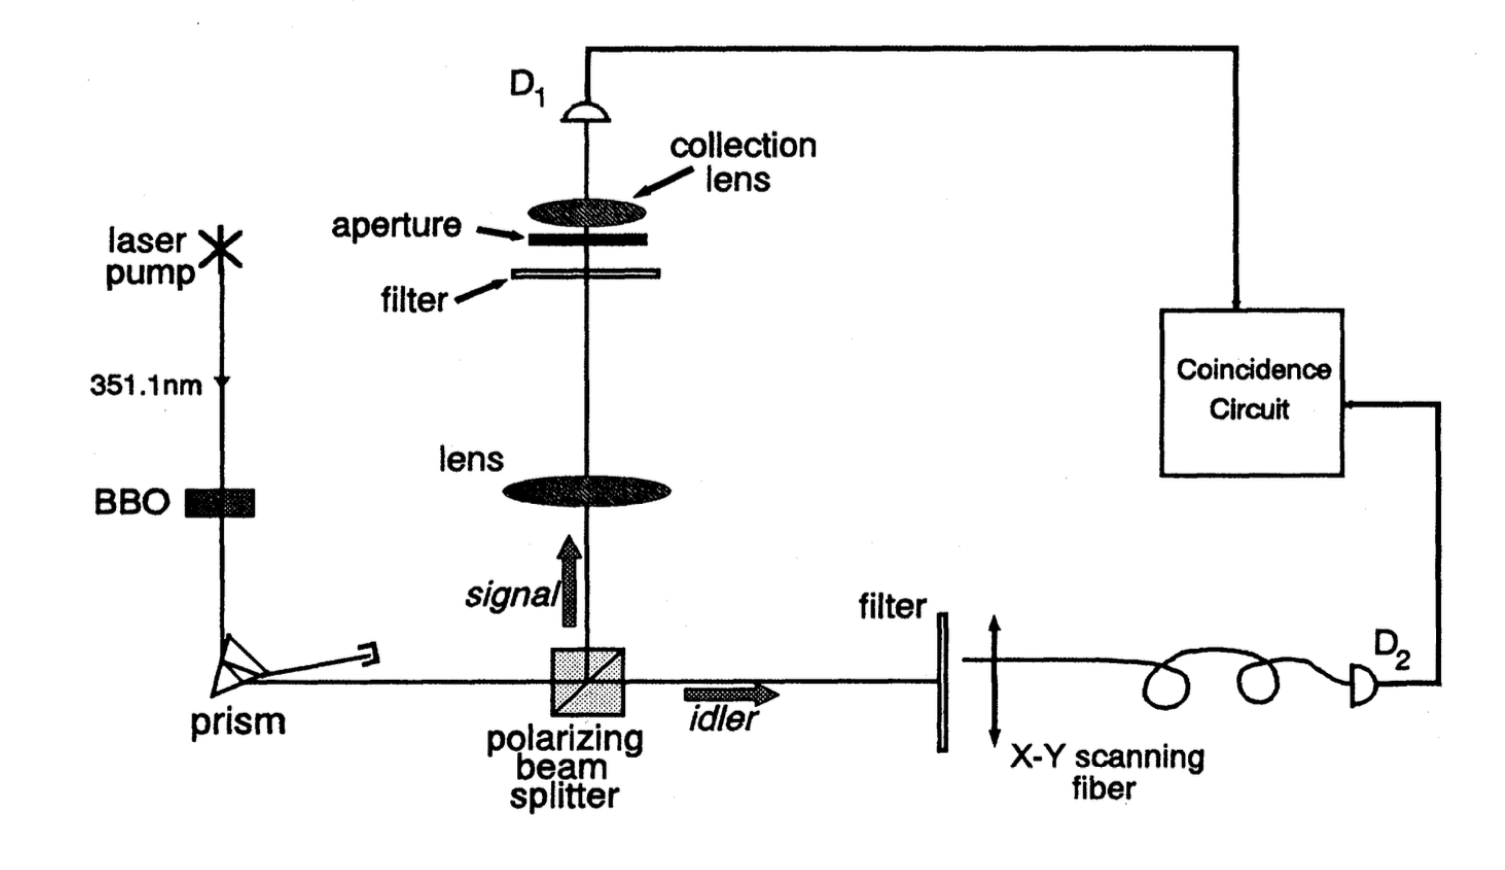
\includegraphics[width=0.75\textwidth]{Figures/pittman.png}
\caption{Schematic of the first "two-photon imaging" experimental setup, used by Pittman\cite{pittman}} 
\label{fig:pittman}
\end{figure}
A continuous wave (CW) laser is used to pump a type-II nonlinear 
crystal to produce pairs of entangled photons. This pairs of orthogonally polarized signal and idler photons are the product
of the nonlinear optical process of spontaneous parametric down-conversion (SPDC).
The pair emerges from the crystal collinearly\footnote{The pairs emerge from the crystal nearly 
collinearly, with $\omega_s \simeq \omega_i \simeq \omega_p / 2$. where the subscript
letter stands for signal, idler and pump respectively}, it is separated by a dispersion prism, 
and then the signal and idler are sent in different directions by a polarization
beam slitting Glan-Thompson prism. 

The reflected signal beam passes through a 
convex lens with a $400mm$ focal length and illuminates an aperture\footnote{The aperture 
consisted of the letters UMBC, University of Maryland Baltimore County.}.
Before the aperture is placed a filter, 
this is a bandwidth spectral filters centered at the
wavelength $702.2 nm$. 
Behind the aperture is the detector package $D_1$. \\
%\begin{figure}[H]
%\centering
%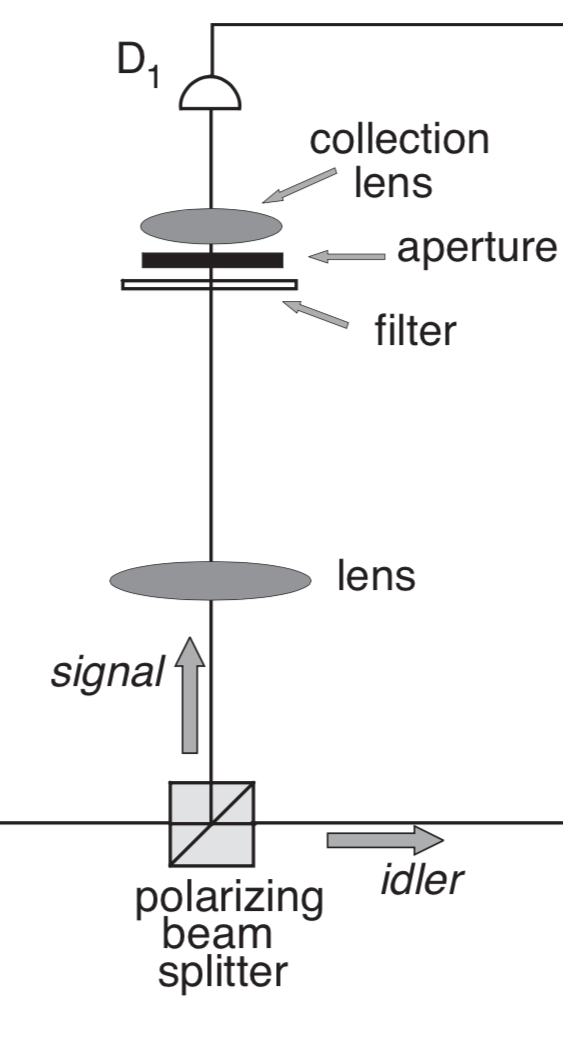
\includegraphics[width=0.24\textwidth]{Figures/signal.png}
%\caption{The reflected photon, called signal} 
%\label{fig:signal}
%\end{figure}


The transmitted idler beam is met by detector 
package $D_2$. The input tip of the fiber is scanned in the transverse 
plane. The counts are sent to a coincidence 
counting circuit with a $1.8ns$ acceptance window.
An important fact of this experiment is the use of a lens(collection lens) in the signal beam that establishes 
an image plane with the definitive point-by-point correspondence object(mask) plane.\\

\subsubsection{Propagation of light through 2-f system}

In order to treat this problem in a more general way it, we need to know 
the state of the biphoton at the output of the crystal:
\begin{equation}
\label{eq:crystal}
\tilde{\Phi}_c(q_c,q_c)=N e^{\left[ -\frac{1}{2}x^T A x + i b^T x \right]}
\end{equation}
Then from this result we can use the fresnel propagation theory to analytically model the biphoton 
propagation in any arbitrary Two-photon Imaging/Lensless Two-photon Imaging setup.This propagation is done 
by determining the Green function of the optical path by which the beams will travel.


\begin{figure}[h]
\centering
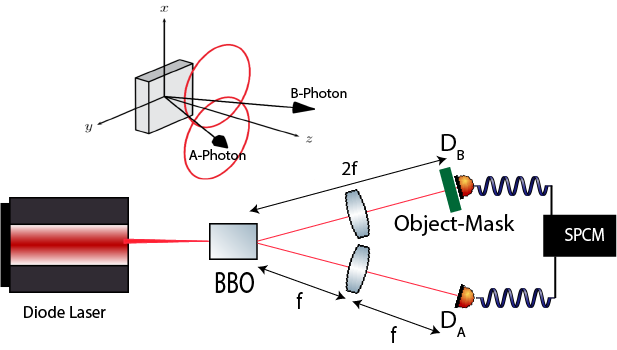
\includegraphics[width=0.75\textwidth]{Figures/simpleTwo.png}
\caption{Simple schematic for a Two-photon Imaging using entangled photons and a 2-f system} 
\label{fig:2f}
\end{figure}
 
Since both path A and B have an identical 2-f system, we are at the called Fourier plane. It is 
well know that when the light goes through this system suffers a Fourier transform\cite{introquantumoptics}. It means that if 
we treated the photons as an ensemble of many oscillating in coherent modes, there is a relation beetwen
the initial $q_c$ initial transverse momentum at the crystal, and the $r_f$ final position of 
the photons. This relation is:
\begin{equation}\label{eq:fourier}
q_{initial}=\frac{2 \pi}{\lambda f} r_{final}
\end{equation}
where $q_{initial}$ is the transverse momentum of the light before the 2-f system, $r_{final}$ is the position of photon
after going through the lens and traveling a 2-f distance. $f$ stands for the focal length of the lenses used and $\lambda$ for the frequency of the coherent mode.\\
The Green function that propagates light with transverse momentum $q$ from the source, to the
Fourier plane located at a position $r_f$ is\cite{green}:
\begin{equation}\label{eq:green}
G(q,r_f) = \int d^2 r_l \int d^2 r_c h(r_f - r_l,f) L_f(r_l) h(r_l - r_c,f) e^{i q \cdot r_c}
\end{equation}
with $r_c$ and $r_l$ denoting the transverse position vectors in the plane of the crystal and the 
lens respectively. $h(r_f - r_l,f)$ and $h(r_l - r_c,f)$ are the Fresnel propagators\footnote{Fresnel Propagator: $h(r,z)=(- \frac{i}{\lambda z})e^{(i \frac{2 \pi z}{\lambda})} \Psi (r,z)$ 
with $\Psi(r,z) = e^{(i \frac{\pi}{\lambda z })r^2}$. } that propagates light from $r_l$ to $r_f$ and 
$L_f (r)=\Psi(r,-f)$ is the thin-lens transfer function associated to a lens\cite{green}.
 \\
Taking advantage of the 2-f system as a Fourier transform to reduce the amount of calculations
, using the relation \ref{eq:fourier}, and after solving the integrals over $r_l$ and $r_c$, equation
 \ref{eq:green} can be written as:
\begin{equation}
\label{eq:greenSolve}
G(q,r_f)=C e^{\frac{i \pi}{\lambda f} r_f^2} e^{\frac{i \lambda f}{4 \pi} q^2} \delta ( q - \frac{2 \pi}{\lambda f}r_f)
\end{equation}
where C is a complex constant and $\lambda $ is the wavelenght of the used light.
Then we can finally propagate  biphoton function
in terms of transverse momenta. Where $\Phi_1 (q_B , q_A )$ is the biphoton after traveling
through two arbitrary optical paths, it can be expressed
in terms of the corresponding Green functions and the
initial biphoton function, equation \ref{eq:crystal}, $\tilde{\Phi}_c(q_c,q_c)$ as:

\begin{equation}\label{eq:final}
\Phi_1 (q_B , q_A )= G_B(q_B,r_B) G_A(q_A,r_A) \tilde{\Phi}_c(q_c,q_c)
\end{equation}
\begin{equation}\label{eq:finalPosi}
\Phi_1 (r_B , r_A )= \int d^2 q_B d^2 q_A \Phi_1 (q_B , q_A )
\end{equation}

where $r_B$ and $r_A$ denotes the photon position in the transverse plane at a 2-f distance from the 
crystal, the subscrip stand for the different path followed by light, Figure \ref{fig:2f}. The $G_B(q_B,r_B)$
and $G_A(q_A,r_A)$ are the green functions for each path, defined as in equation \ref{eq:greenSolve}, they are:
\begin{equation}\label{eq:B}
G_B(q_B,r_B)=G(q_B,r_B) \times T(r_B) 
\end{equation}
\begin{equation}\label{eq:A}
G_A(q_A,r_A)=G(q_A,r_A)
\end{equation}
Where $T(r_B)$ is the transfer function of the object, which is only present at the $B$ path, Figure \ref{fig:2f}.
Gathering all the previous results we can obtain $\Phi_1 (r_B , r_A )$. This is done by replacing
Eq. \ref{eq:B} and \ref{eq:A} into Eq. \ref{eq:final}, then evaluating the integrals over the transverse 
momentums, Eq. \ref{eq:finalPosi}, we obtain:
\begin{equation}\label{eq:finalBiphoton}
\Phi_1 (r_B , r_A )=C^2 T(r_B) \Phi (\frac{2 \pi}{\lambda f}r_B, \frac{2 \pi}{\lambda f}r_A)
\end{equation}

This function describes the biphoton at the planes of the object and the scanning detector. It shows 
that the biphoton at the 2F plane as a function of $r_B$ and $r_A$. If we take a closer look, this result
enable us to compute the biphoton at the 2-F plane by using Eq \ref{eq:quadratic} without the need to actually calculate its propagation, just by 
evaluating it with the Fourier relationship, \ref{eq:fourier}. This is specially usefull when we try to 
simulate this on a computer, the amount of calculations is significantly reduced by this fact.

As described at the beginning of this Section \ref{twoPhotonImaging}, we lose all the spatial information 
about the photon that interacts with the Object, and this is done by placing a bucket detector that
gathers all light and send it to a multimode optic fiber, without saving any information about the position
of the photons in this path $B$. From the mathematical point of view, the bucket detector is modeled
as: $\Phi_1 (r_A) = C^2 \int d^2 r_B T(r_B) \Phi (\frac{2 \pi}{\lambda f}r_B, \frac{2 \pi}{\lambda f}r_A)$.
Using the fact that the coincidence counts that will be measured by the Detectors will be 
proportional to the magnitude square of the resulting biphoton function $\Phi_1 (r_A)$\cite{introquantumoptics}.
\begin{equation}\label{eq:S}
S(r_A) \propto |  \int d^2 r_B T(r_B) \Phi (\frac{2 \pi}{\lambda f}r_B, \frac{2 \pi}{\lambda f}r_A) |^2
\end{equation}
Where $S(r_A)$ is the function that describes de coincidences counts between de detectors $D_B$ and 
$D_A$ in Figure \ref{fig:2f}. $S(r_A)$ is a function of the spatial positions, $(x_A,y_A)$
 of the detection plane at $D_A$. This function $S(r_A)$ have the expected behaviour described
by $R_{BA}(\vec{\rho_A})$ in Eq. \ref{eq:coincidences}, where the second-order correlation function in this 
case is $\Phi (\frac{2 \pi}{\lambda f}r_B, \frac{2 \pi}{\lambda f}r_A)$, as we said, the function
containing all the informations about the correlations between the pair of down-converted photons. 
Moreover, Equation \ref{eq:S} indicates that the form of $\Phi(q_B,q_A)$ determines if $T(r_B)$ can
be recovered in the coincidence count. Additionally, the type of spatial correlation in $\Phi(q_B,q_A)$
defines the orientation of the image obtained.

\subsubsection{Two-photon Imaging Using Chaotic Sources}

In principle the term "thermal radiation" should refer only to radiation coming 
from a blackbody in thermal equilibrium at some temperature T. But with this realisation of thermal radiation
we have to face some characteristics of true thermal fields. Thermal radiation is also referred as chaotic light, 
which have extreme short coherence time. This is because a thermal source contains a large number of independent sub-sources,
such as the trillions of atoms or molecules.These atomic transitions that can be identical or different
act like sub-sources, that emit light into independently and randomly. 



\begin{figure}[h!]
\centering
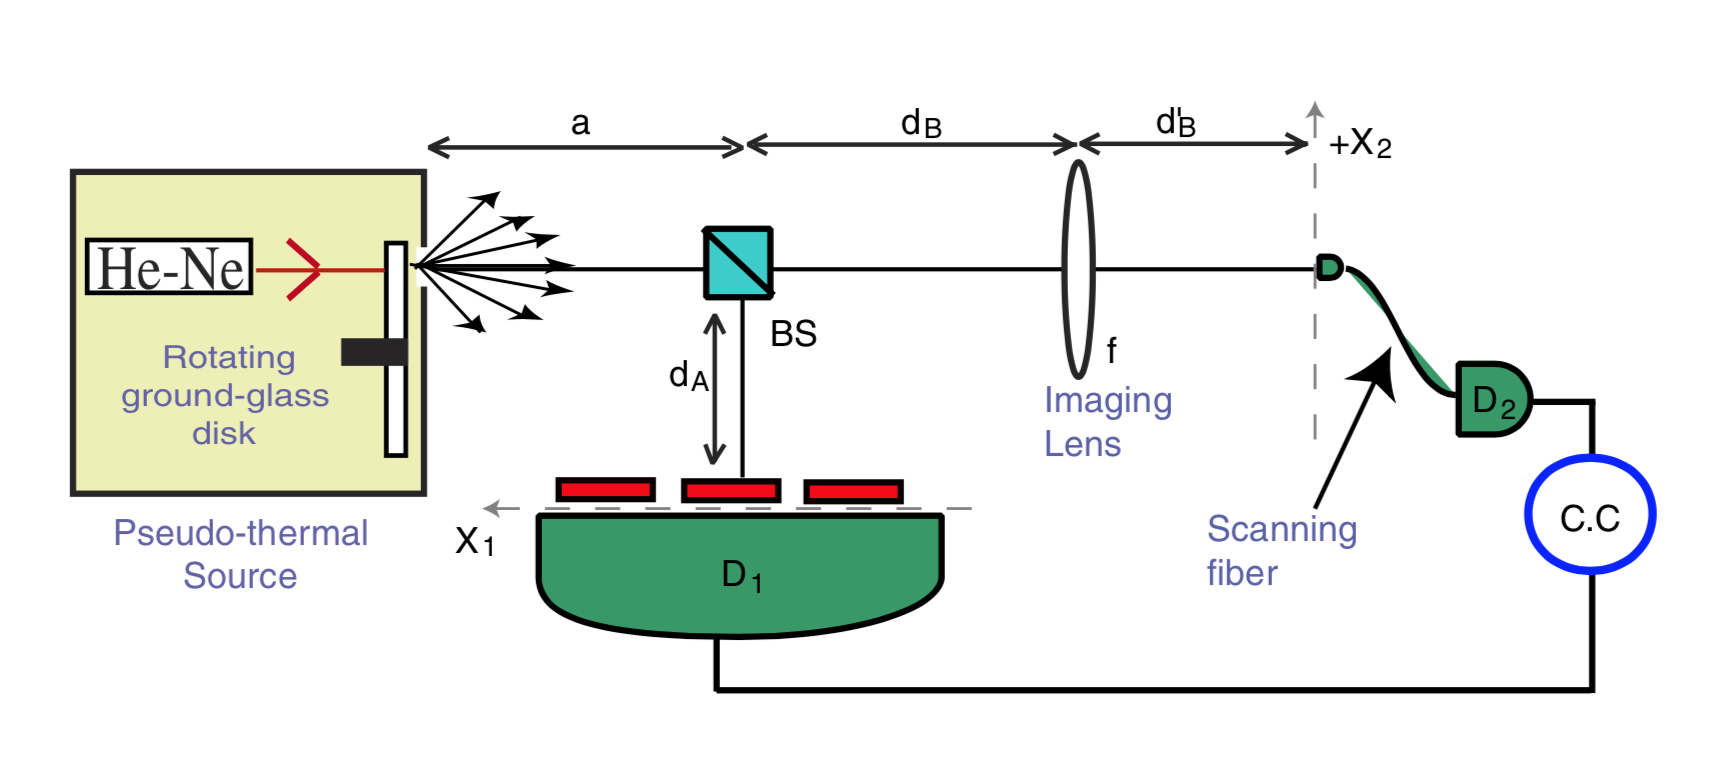
\includegraphics[width=0.6\textwidth]{Figures/thermalSetup.png}
\caption{Experimental setup for the Two-photon imaging using thermal light, taken from \cite{thermalAlejandra}} 
\label{fig:thermalSetup}
\end{figure}
The source light in Figure \ref{fig:thermalSetup} is the one developed by Martinssen and Spiller\cite{intensity}
which is the most commonly used among the pseudothermal fields. A  coherent laser radiation is focused on a rotating ground glass disk, 
the scattered radiation is chaotic with a Gaussian spectrum. After this, a nonpolarizing beam
splitter (BS) splits the radiation in two distinct optical pths, In the reflected arm an object, with 
transmission function $T(r_1)$, is placed ar a distance $d_A$ from the BSand a bucket detector ($D_1$)
is just behind the object. In the transmitted arm an imaging lens, with focal lenght $f$, is placed at a 
distance $d_B$ from the BS, and a multimode optical fiber ($D_2$) scans the transverse plane
at a distance $d'_B$ from the lens. The output pulses from the two single photon counters are sent 
to an electronic coincidence circuit to measure the rate of coincidence counts.

Once again we expect the joint-detection counting rate between photodetectors $D_1$ and $D_2$ to behave
like the one described in Eq. \ref{eq:coincidences}. But thos rate this coincidence counts is governed
by the second-order Glauber correlation function \cite{glauber}:
\begin{equation}
G^{(2)} (\vec{r}_1; \vec{r}_2) \equiv \langle E^{(-)}_1(\vec{r}_1)E^{(-)}_2(\vec{r}_2) \times E^{(+)}_2(\vec{r}_2)E^{(+)}_1(\vec{r}_1) \rangle
\end{equation}
where the $E^{(-)}$ and $E^{(+)}$ are the negative-frequency and the positive-frequency field operators describing the detection events at the
locations $\vec{r}_1$ and $\vec{r}_2$. The transverse second-order correlation correlation function 
for a thermal source is given by \cite{thermalAlejandra}:
\begin{equation}\label{eq:thermal}
G^{(2)}_{\textit{thermal}}(\vec{r}_1; \vec{r}_2) \propto \sum_{\vec{q}} |g_1(\vec{q},\vec{r}_1)|^2
\sum_{\vec{q}'} |g_2(\vec{q}',\vec{r}_2)|^2 + |\sum_{\vec{q}} g_1^*(\vec{q},\vec{r}_1) g_2(\vec{q},\vec{r}_2)|^2
\end{equation}
where $\vec{r}_i$ is the transverse position of the detector $D_i$, $\vec{q}$ and $\vec{q}'$
are the transverse components of the momentum vectors, and $g_i(\vec{q},\vec{r}_i)$ is the Green's function 
associated with the propagations of the field with transverse momentum $\vec{q}$ from the source, 
to the position $\vec{r}_i$ at the detection plane defined by the detector $D_i$. $g_i(\vec{q},\vec{r}_i)$ is defined in a similar way 
as in Eq. \ref{eq:green}.

It is important to note that there are two main differences with respect to the SPDC case: 
First the presence of a background noise (first term of Eq. \ref{eq:thermal}), which does not exist for SPDC. Second,
the possibility of writing the second term of Eq. \ref{eq:thermal} as a product of the first order correlation
functions, $G^{(1)}_{12}G^{(1)}_{21}$, while there is no way to write the biphoton produced by the 
SPDC as a product of other correlations. Also this term $|\sum_{\vec{q}} g_1^*(\vec{q},\vec{r}_1) g_2(\vec{q},\vec{r}_2)|^2$
Is the interference of intensities of a incoherent statistical assemble of randomly distributed photons.


Following the proces done in \cite{thermalAlejandra}, it can be shown that for any values of distances
$d_A$, $d_B$ and $d_{B}'$ which obey the equation:
\begin{equation}
\frac{1}{d_B - d_A} + \frac{1}{d_{B}'} = \frac{1}{f}
\end{equation}
which clearly has the form on a thin-lens equation, defining a point-to-point correspondence between imaging and object plane.
Then Eq. \ref{eq:thermal} can be simplified as:
\begin{equation}
G^{(2)}_{\textit{tot}}(\vec{r}_2) \propto N + | T \left( \frac{d_A - d_B}{d_{B}'} \vec{r}_2 \right) |^2
\end{equation}
where $T ( \frac{d_A - d_B}{d_{B}'} \vec{r}_2 )$ is the object transmission function ($T(\vec{r}_1)$)
reproduced on the $D_2$ plane. Thanks to this result we can conclude that a thermal source allows reproducing
in coincidence measurements the two-photon image of an object, similarly to the SPDC case, except for a 
constant background noise, where $N$ is proportional to it.


It is possible to establish an analogy
between classical optics and entangled two-photon optics:
the two-photon probability amplitude plays in entangled
two-photon processes the same role that the complex amplitude
of the electric field plays in classical optics  \cite{thermalAlejandra}. 
% Chapter Template

\chapter{Experimental Setup} % Main chapter title

\label{Chapter3} % Change X to a consecutive number; for referencing this chapter elsewhere, use \ref{ChapterX}
In the following chapter we will look in detail the components of the experimental 
setup and its stages. This experimental setup located on the optical table of the 
Quantum Optics Laboratory
%----------------------------------------------------------------------------------------
%	SECTION 1
%----------------------------------------------------------------------------------------
\section{SPDC Setup}
Following the treatment made in the previous chapter. The first ingredient is the SPDC light, to obtain pair of photons
 the experimental setup shown in Figure \ref{fig:SPDC}. From here we will star describing each of the components
presented.


\begin{figure}[h!]
\centering
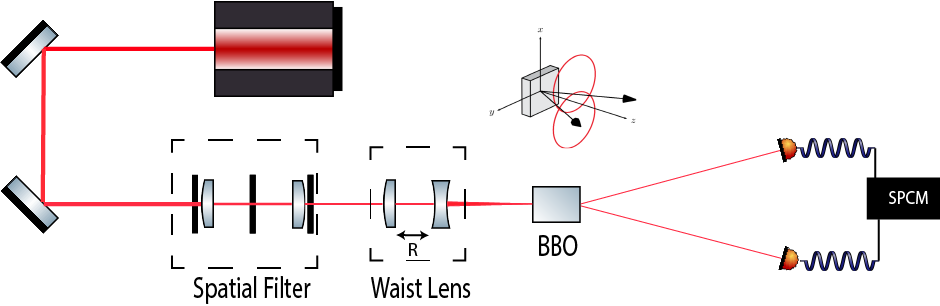
\includegraphics[width=0.8\textwidth]{Figures/SPDC.png}
\caption{Experimental Setup for the SPDC light Source} 
\label{fig:SPDC}
\end{figure}

\subsection{Diode Laser}
Before having pair of correlated photons, we start by having a coherent light source, 
for this experiment we use a Diode Laser that delivers a continuous wave(CW) at 
$\lambda = 406,101 nm$ and $\Delta \lambda = 4 nm$. 
The laser model No. DL 405-200 delivers light at 200 mW with a beam diameter 
of 1.5 mm and a beam Divergence\footnote{The beam divergence is an angular measure of the increase in beam diameter with distance from the original optical aperture}
 1.2 mrad. 

\begin{figure}[h!]
\centering
{  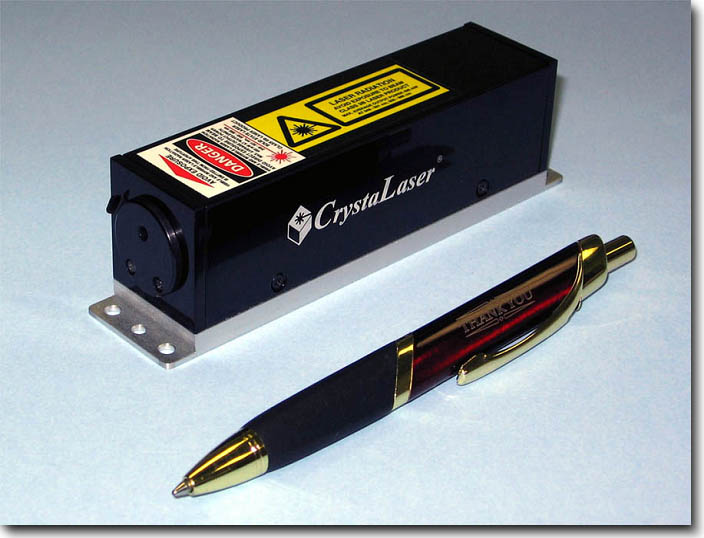
\includegraphics[width=0.45\textwidth]{Figures/diodeLaser.jpg} }
{  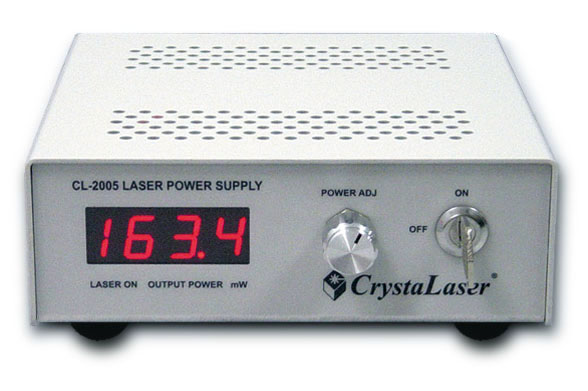
\includegraphics[width=0.45\textwidth]{Figures/diodeLaserControl.jpg} }
\caption{Image of the Diode Laser and it's control module, Taken from \cite{crystalLaser}}
 \label{fig:diodeLaser}
\end{figure}




\subsection{Mirror}
As seen in Figure \ref{fig:SPDC} we redirect the laser beam two times, for doing
so we use a pair of mirrors. For this kind of experiments, when the efficiency 
of the optical elements is really important, it is important to use the correct type
of mirror, we want a mirror that reflects most of the light. For this reason, depending
on the wavelength it is posible to find mirrors and lenses with different types of 
coating. Mirror and Lenses have a thin layer that is more efective for a range 
of wave lengths.

In Figure \ref{fig:mirror} we can see a Mirror and the base used to place it, it is posible
to manipulate the direction in which the mirror will reflect the light,  we can do this 
by manipulating the screws, each one moves the reflected laser in one direction. 
In the experimental setup we use two mirror to change the direction two times, this is because 
using just one could be more complicated when aligning the rest of optical elements. 
When two mirror are used, we have more possibilities, 4 in total. The advantage 
of having more possibilities is that the manipulation can be more precise.
\begin{figure}[h!]
\centering

 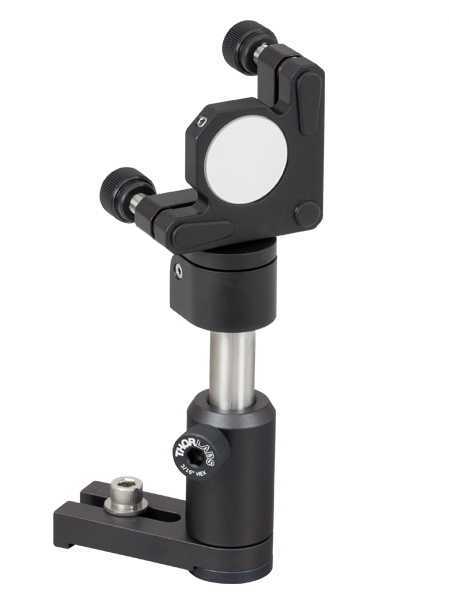
\includegraphics[width=0.3\textwidth]{Figures/mirror.jpg}
\caption{Mirror and the cavity mount} 
\label{fig:mirror}
\end{figure}

\subsection{Spatial Filter}
A laser beam can be characterized by measuring its spatial intensity profile at points perpendicular to its direction of propagation. 
The spatial intensity profile is the variation of intensity as a function of distance from the center of the beam, in a plane perpendicular to its direction of propagation.
\begin{figure}[h!]
\centering
{  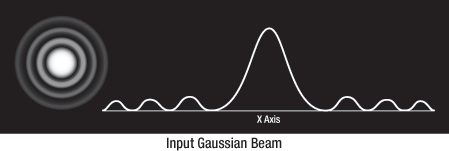
\includegraphics[width=0.6\textwidth]{Figures/inputBeam.png} }
{  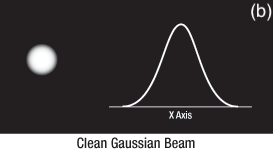
\includegraphics[width=0.6\textwidth]{Figures/outputBeam.png} }
\caption{The spatial intensity profile before and after the spatial filtering process , Taken from \cite{thorlabs}}
 \label{fig:inputOutputBeam}
\end{figure}
In Figure \ref{fig:inputOutputBeam} we se see the input gaussian beam 
and how its intensity fluctuates around the x axis. The output desired beam after going through the spatial filter is then shown.
The simplest arrangement to achieve this output spatial intensity profile is show in the Figure \ref{fig:spatialFilter}, 
where at the end we have a beam which intensity strength falls off transversely following a bell shaped curve that's symmetrical around the central axis.
\begin{figure}[h!]
\centering
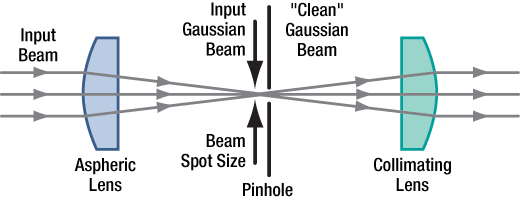
\includegraphics[width=0.55\textwidth]{Figures/spatialFilter.png}
\caption{Basic elements of a Spatial Filter. In our experiment we use a Aspheric Lens of $f=30 mm$(LA1805-A), a pinhole of $50 \mu m$ and a collimating lens of $f=60 mm$(LA1134-A). Taken from \cite{thorlabs}} 
\label{fig:spatialFilter}
\end{figure}
Taking a closer look at the input Gaussian beam in Figure \ref{fig:inputOutputBeam} we may recognise a diffraction pattern, the well known Airy disks. 
However, when we measure this spatial profile directly from the diode laser, we find out that it doesn't follow that behaviour, on the contrary 
it follows a more random spatial profile. This ramdom spatial profile is a result of the randomnes in the
quantum emissions and absorptions that are happening at the exited atoms at the diode laser\cite{hecht}.

In order to have this spatial intensity profile at the input of the lens arrangement, Figure \ref{fig:spatialFilter},
we put a circular aperture with the help of a iris, Figure \ref{fig:iris}, before the $f=30.0 mm$ lens. Another optional iris is placed after the $f=60.0mm$ lens.
\begin{figure}[h!]
\centering
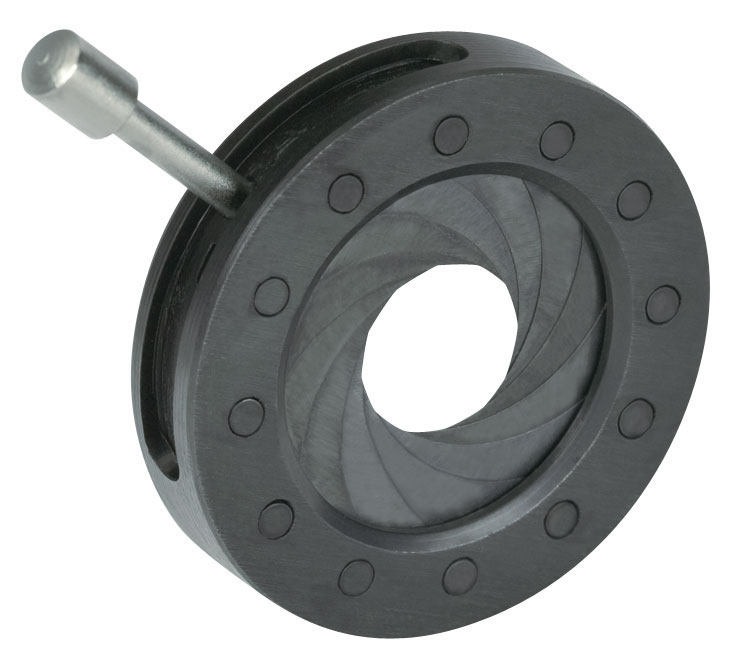
\includegraphics[width=0.25\textwidth]{Figures/iris.jpg}
\caption{This helps to form circular apertures of variable radius} 
\label{fig:iris}
\end{figure}


IN HERE I MAY TALK ABOU THE M FACTOR, QUALITY PARAMETER OF GAUSIAN BEAMS $M^2$ 
Power $200mW$

\subsection{Waist Lens}
After successfully achieving a Gaussian profile, which is important for the reasons described in Section \ref{sec:spatialCorrelations}.
After the spatial filter, we need a way to control the pump waist, but we need to do it in a way not too complicated, that 
doesn't imply too many changes in the experimental setup. Putting a  lens in the propagation direction with certain focal lenght $f$ will define a zone around
the distance f called \textit{Focus depth}\cite{hecht}, where in the middle we find the narrowest point of the beam.
The radius of this zone is:
\begin{equation}
 W_0=\frac{\lambda f}{\pi W_B}
\end{equation}
Where $W_B$ is the initial waist beam. 
In Figure \ref{fig:waist} we see this behaviour, this zone is produced around the distance $f$ and
the radius $W_0$ is a function of $f$ and $W_B$. making that if we want to change
$W_0$ we need to use a different lens with $f'$ and also the \textit{Focus depth}
will be at a different distance.

\begin{figure}[h!]
\centering
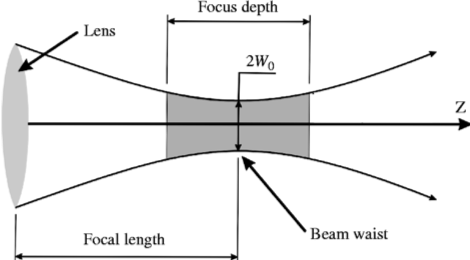
\includegraphics[width=0.35\textwidth]{Figures/waist.png}
\caption{Effect of lens on a Gaussian beam} 
\label{fig:waist}
\end{figure}

If we want to focus the beam at a fixed distance $F$, using this method to control the pump waist is not practical. 
Every different lens we would use will make this waist $W_0$ at a differents distances $f$. It is necessary to find a \textit{Waist lens}
that make us a $W_0$ at a transverse plane located in a fixed position $F$ from the \textit{Waist Lens}. 
In Figure \ref{fig:fixed} we present a special lens, consisting in an arrangment of two lenses, a positive 
and negative one respectively, separated a distance $d_0$ from each other.
\begin{figure}[h!]
\centering
 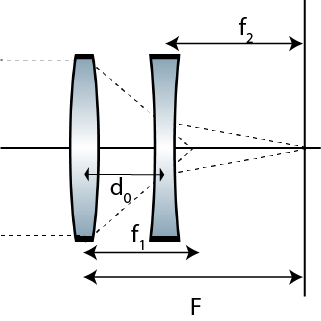
\includegraphics[width=0.65\textwidth]{Figures/fixed.png}
\caption{Composition of lenses to control the Pump Waist at a Fixed distance $F$} 
\label{fig:fixed}
\end{figure}
Where we can define a \textit{effective focal length} $F$ as a function of  $f_1$ and $f_2$, the focal lengths of the positive and negative lenses 
respectively. With the constrain that $d_0 < f_1$, $F$ reads:
\begin{equation}
F=\frac{f_1 |f_2|}{|f_2|-f_1+d_0}.
\end{equation}
This new effective focal length is crucial in the realisation of this experiment, as described before, we are interested in observing the effect 
in the reconstructed image using different spatial correlations. This is done by changing the pump waist of the laser that is focused on the crystal.
It is not experimentally practical to be changing the crystal position, it would mean to change the position of all the optical elements that 
follows. For this reason, it is perfect to be able to achieve the desired pump waist just by changing the relative separation of two lenses. 


\subsection{BBO(Beta Barium Borate) Crystal}
The Beta Barium Borate (BBO) is an inorganic compound, with chemical formula $\beta$-BaB$_{2}$O$_4$. This crystal is a
nonlinear optical media commonly used. It is also a birefringent\footnote{Birefringence is a optical property of some materials of 
having a refractive index that depends on the polarisation and the propagation of light\cite{hecht}} material and its transmission regions extends
from $189nm$ to $3500nm$\cite{bbo}.
The type-II crystal is mounted is such way that the input and output plane are fixed, Figure \ref{fig:bbo}(a). In particular the input plane is at $F$ from 
the \textit{waist lens} presented in the previous section, the power of the pump at this point is $\sim 60mW$. In Figure \ref{fig:bbo}(b) is a schem of 
the noncolinear configuration at the output plane of the crystal.

\begin{figure}[h!]
\centering
{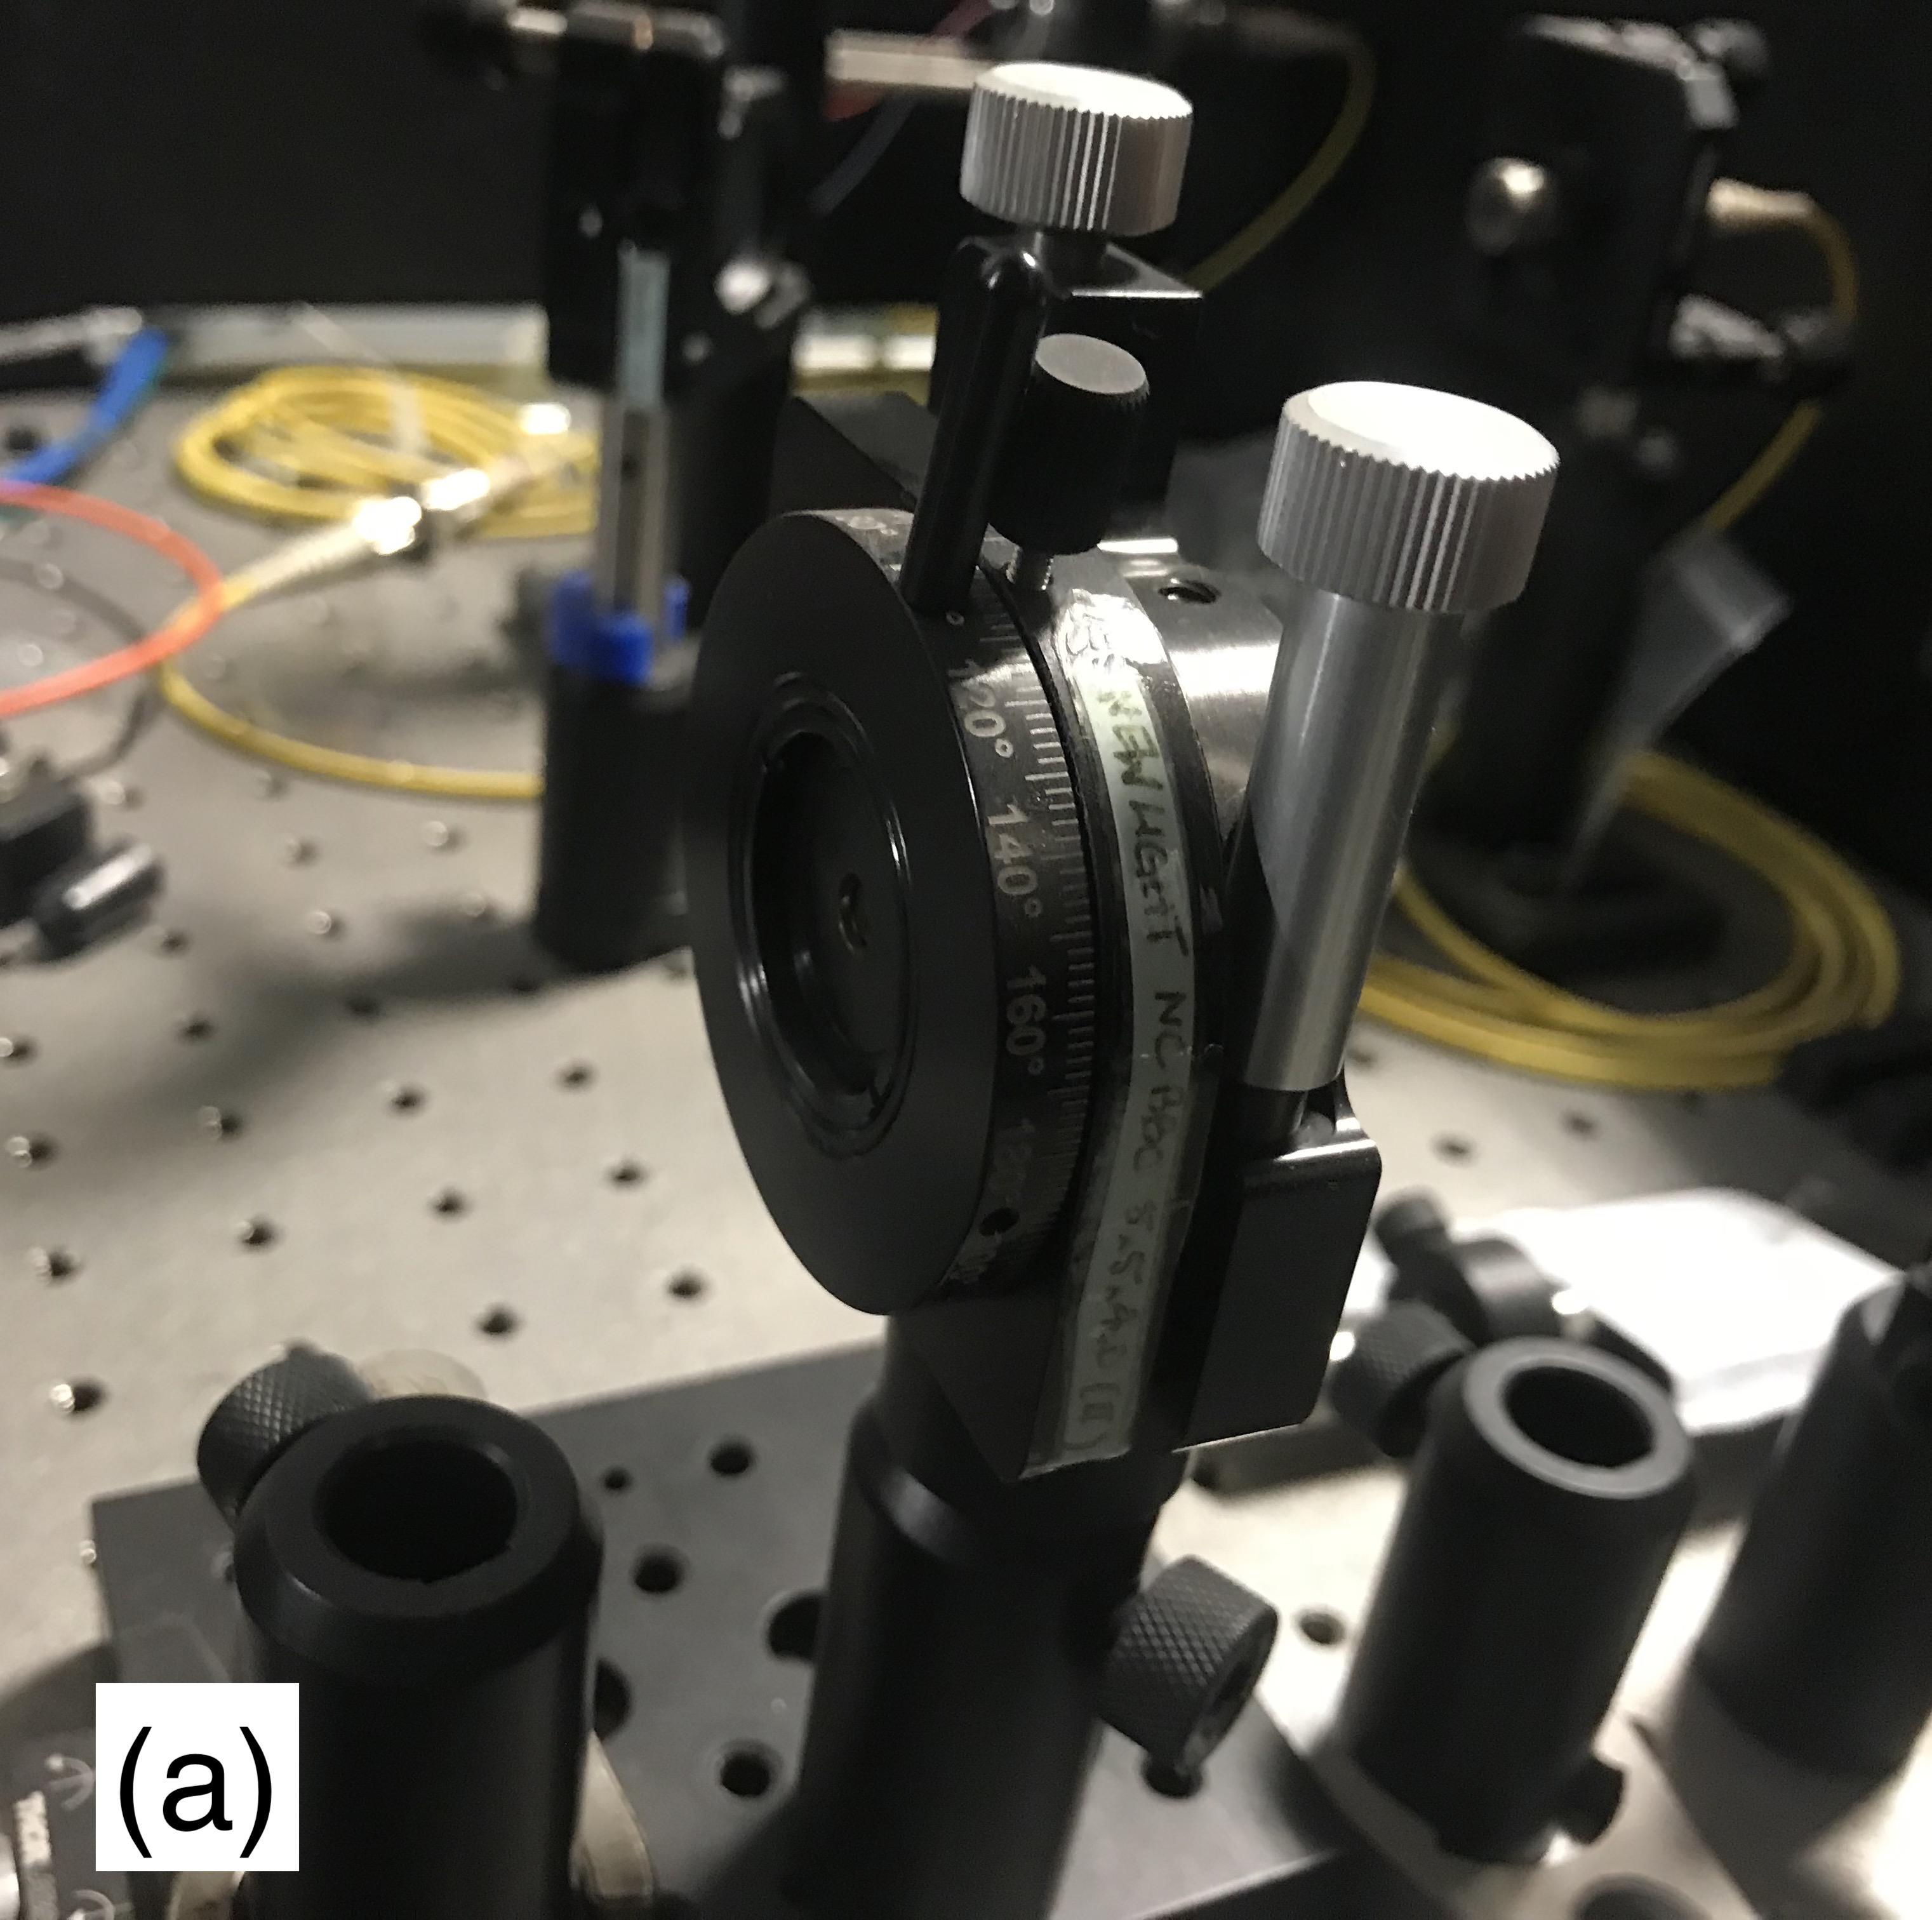
\includegraphics[width=0.35\textwidth]{Figures/bbo.jpg}}
{  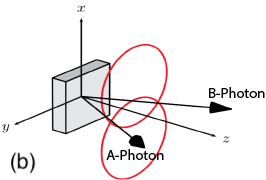
\includegraphics[width=0.5\textwidth]{Figures/aPhotonBPhoton.png} }
\caption{(a):Actual BBO crystal used in experiment. (b): the noncolinear configuration presented in this experiment}
 \label{fig:bbo}
\end{figure} 

At this point we have as a result of the SPDC process a pair of entangled photons, which have an strong correlation. This correlation is 
the feature in which we are interested on. We need to observe the shape of this correlations functions and the next section will focus 
on the experimental setup that will allow us to observe this.



\section{Spatial Correlations Measurement Setup}
From this point we will talk about a pair of correlated photons, that will come from the output plane of the BBO 
crystal, for historical reasons this photons are labeled as \textit{signal} and \textit{idler}. Nevertheless, to keep the same notations used through 
this monograph, this photon are going to be labeled as A-photon and B-photon, depending on which path they follow, in Figure \ref{fig:spatialSetup}
we can see the experimental setup for measuring the spatial correlations, and the different paths the light follows.

\begin{figure}[h!]
\centering
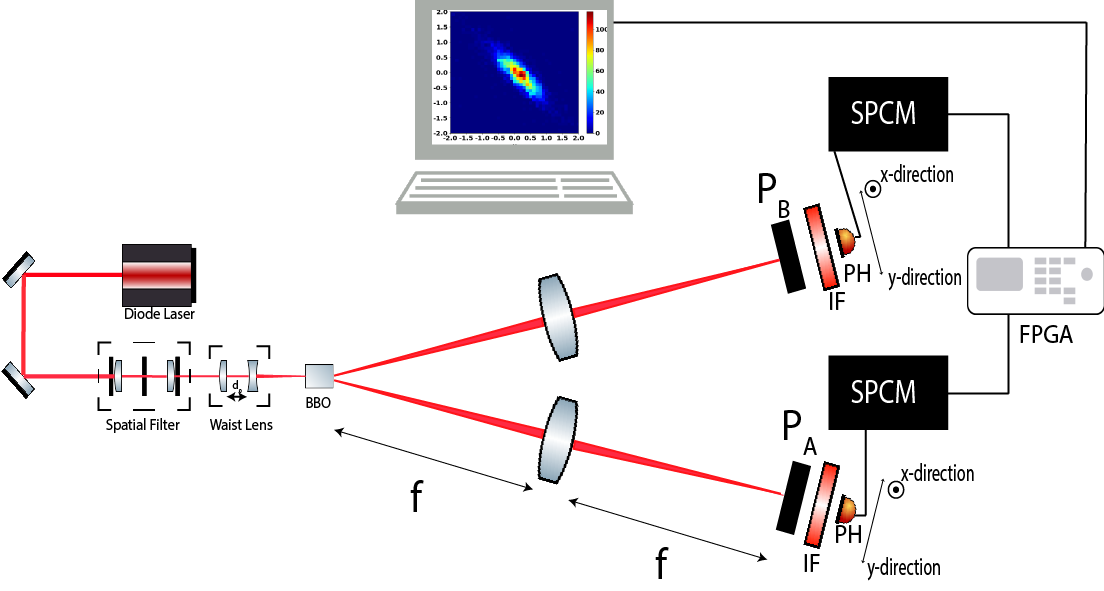
\includegraphics[width=1\textwidth]{Figures/spatialCorrelationSetup.png}
\caption{Experimental Setup for Obtaining the spatial correlations of a pair of down-converted photons} 
\label{fig:spatialSetup}
\end{figure}

\subsection{Lens (Fourier Plane)}
The next optical element that the pair of correlated photons find in their path is a pair of lenses. This pair of lenses are located at a
distance $f$ from the crystal. They define a $2f$ system and place a Fourier plane at a $2f$ distance from the crystal. As discused before, 
this plane is important because of the relation between the transverse momentum of the light before the 2-f system, and the photon 
position after de system, Eq. \ref{eq:fourier}. We use a lens(LA1708) of $f=200.0mm$ in front of each \textit{A} and \textit{B}. 


\subsection{Polariser}

We are interested in just a pair photons, $\Phi(\vec{q}_B,\Omega_B;\vec{q}_A,\Omega_A)$, that are polarised in certain direction. In order to filter the others
photons $\Phi(\vec{q}_A,\Omega_A;\vec{q}_B,\Omega_B)$, we place a pair of polarisers at both paths. A polariser is an optical element that filter light, it filters
light depending on the direction of the electrical field. We used a pair of Polarisers(WP25M-UB), which consist of an array of parallel metallic
wires sandwiched between glass with certain coating for better transmission.

\subsection{Interferometer Filter}
As pointed out in Section \ref{sec:spatialCorrelations}, in order to observe the transverse
correlations, the frequency information has to be traced out. For doing so, we placed a 
pair Interferometer filters. This optical elements have the special feature that only transmits 
light that comes throught in certain range of frequencies. To do this filtering we used a spectral filter(FB810-10) that only transmits the light that comes
with $\lambda =810 \pm 2nm$.

\subsection{Detection Module}
To observe the spatial correlations we have to be able to measure light that is propagating
in the z-direction. Figure \ref{fig:scan} shows the plane that is being scanned, where each 
square have a $x_i$ and $y_j$ position, ${i,j}$ goes from $0$ to $N$. With the help of a motorised translational stages, we can make this $N$ steps. we can 
control the movement of a pin hole detector, which consists in a single mode optical fiber tip. The translationas stages are controlled 
by Arduinos, this enable us to do the scan in a complete automated way.
\begin{figure}[h!]
\centering
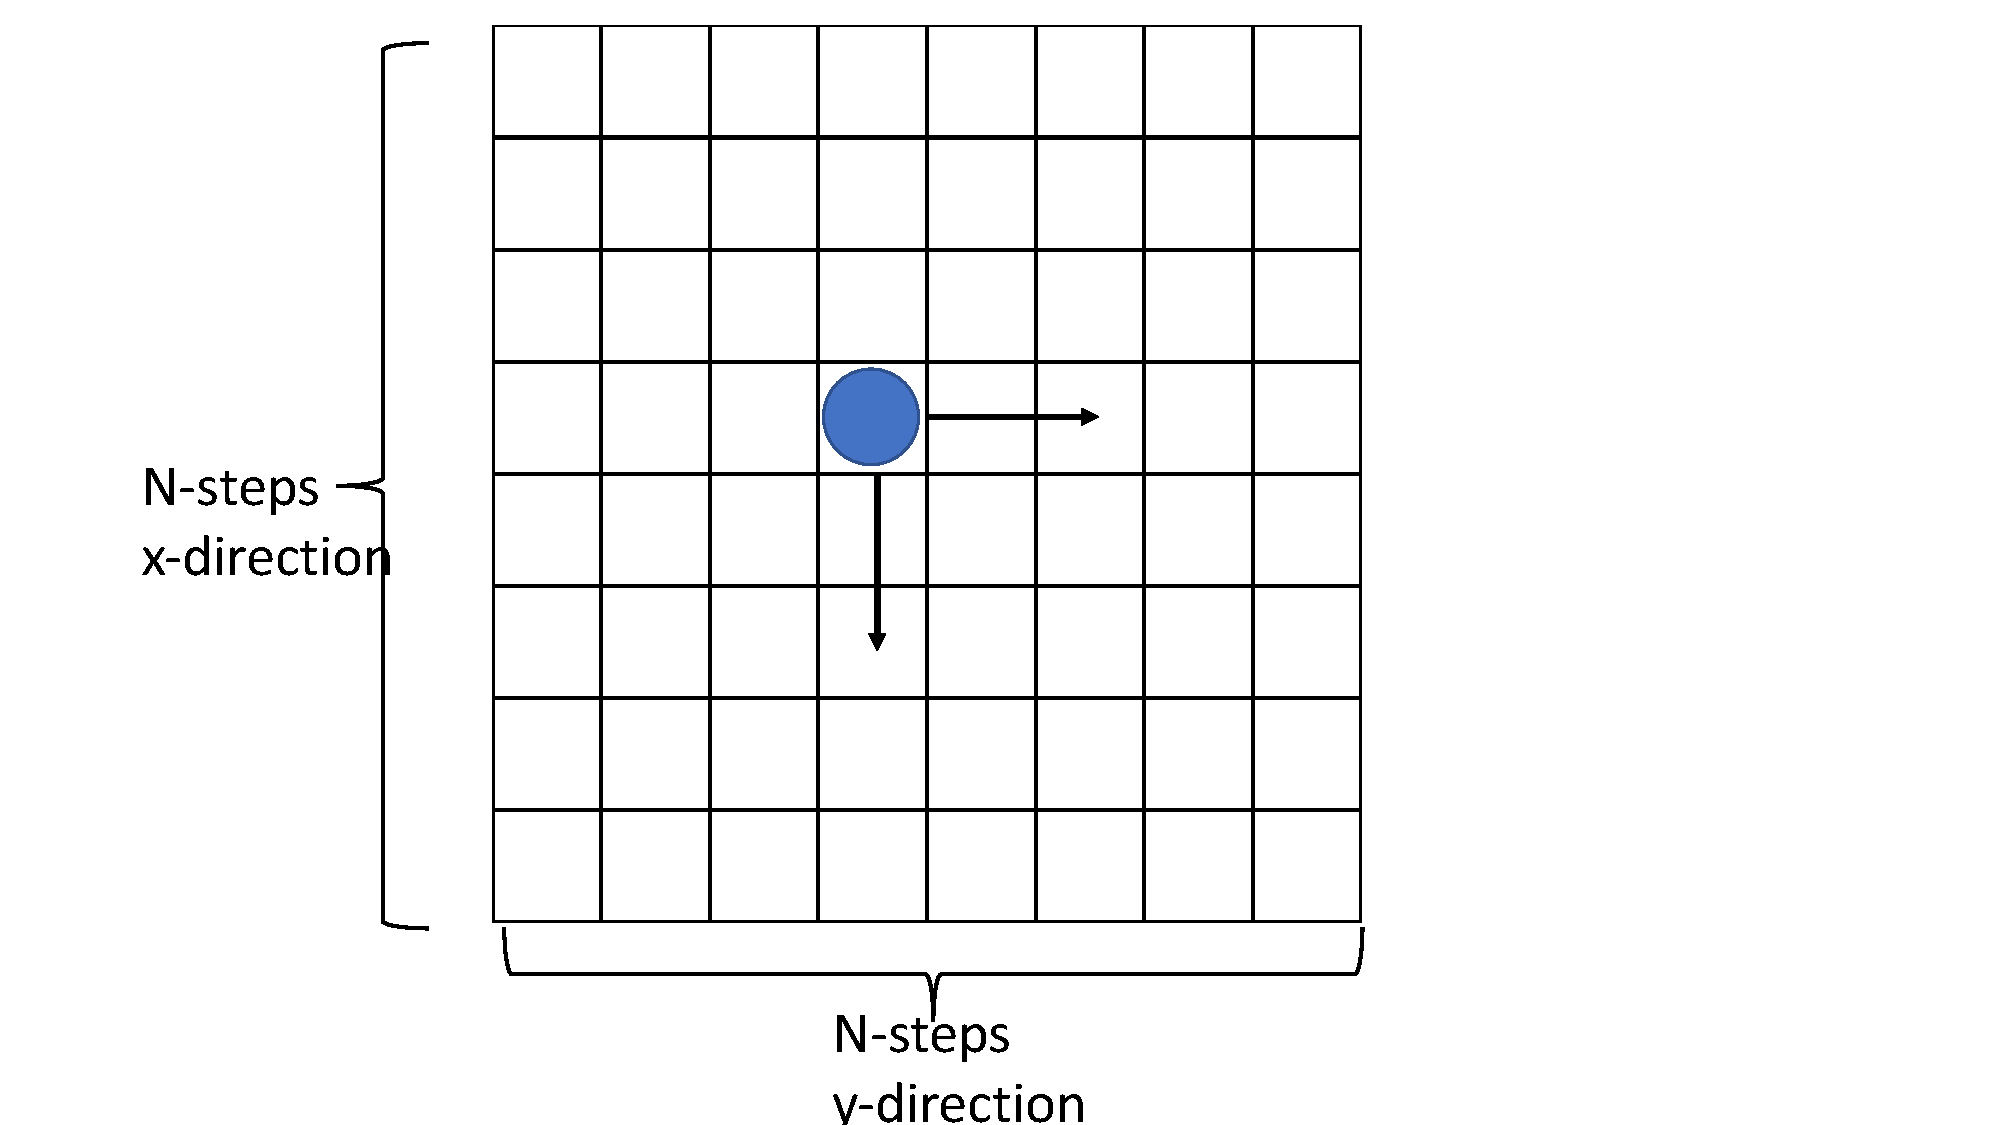
\includegraphics[width=1\textwidth]{Figures/scan.pdf}
\caption{The plane that is being scanned by the fiber tip, it is a $4x4mm$ square, that
can be scanned in N steps, where N is defined by us} 
\label{fig:scan}
\end{figure}

Another feature that is easily controlled, is the exposure time. It means we can set how many seconds, is going to be the fiber tip at
every ($i,j$) position. A greater time means more photon counted, and with a bigger amount of data of photons
counted per position, the means values per position gives a better image, with better contrast. The places where we don't have photons 
tend to have a low mean value of photons counted, while the more intense places keep counting, hence having bigger means values.
The ($i_B,j_B$) position and ($i_A,j_A$) position are related with $\vec{q}_B=(q_i,q_j)$ and $\vec{q}_A=(q_i,q_j)$ in Eq \ref{eq:quadratic} 
$\tilde{\Phi}(\vec{q}_B,\vec{q}_A)$, respectively. The spatial correlation we seek to observe. When taking a Two-photon imaging we already deduce in the 
previous Chapter that the image is going to be related with $R(\vec{r}_A)$ from Eq. \ref{eq:R}, where the ($i_A,j_A$)
 position is related with $\vec{r}_A=(x_i,y_j)$.






\subsection{Single Photon Counting Module(SPCM)}

Light is transmitted through an optic fiber from the pin hole detector to the SPCM. This 
consists in a self-contained module that detects single photons of light over the $400nm$ to $1069 nm$
wavelength range. The module used  is SPCM-AQRH-13, and it uses a unique silicon avalanche photodiode (SLiK) with a detection efficiency of more than 65\%\cite{spcm}.
The result signal coming from the SPCM are pulses where each one represents one photon.
\begin{figure}[h]
\centering
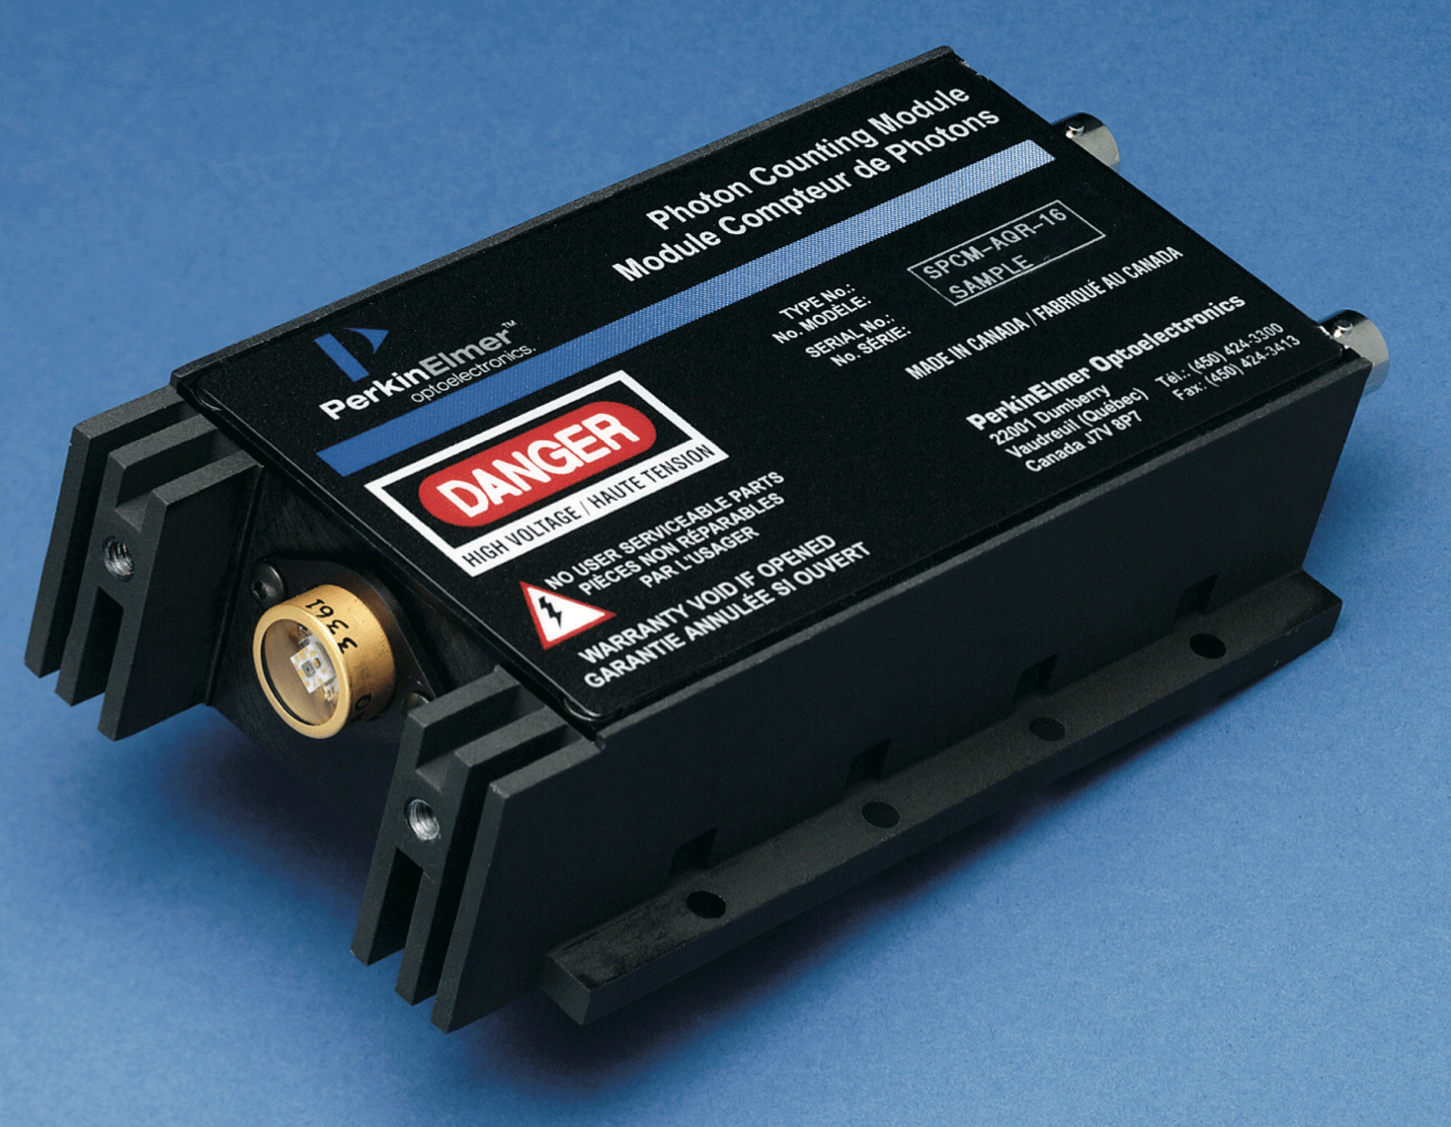
\includegraphics[width=0.35\textwidth]{Figures/spcm.png}
\caption{Single Photon Counting Module} 
\label{fig:spcm}
\end{figure}


\subsection{Field-programmable gate array(FPGA)}
Both \textit{A} and \textit{B} pulses from the respective SPCM goes to the same Field-Programmable Gate Array (FPGA). This
FPGA (ZestSC1) is programmed
to count the photon coincidences, this means that the FPGA is fast enough to detect and separate pulses from photons 
that are time-separated. 




\subsection{Computer(Data Analysis)}
LabvVIEW is used to control the detection module, and also, to recibe and translate the information
from the FPGA. It deliver the single and coincidence counts for every position in the 
scan grid, Fig. \ref{fig:scan}. Using this information is only matter of use any way to handle
this data and generate the graph for single and coincidence counts. Through this monograph
it has been used the python language and the matplotlib library to generate them.


\section{Two-Photon Imaging Setup}
For the Two-photon imaging process we no longer have spatial information about the  B-photon after it interacts
with the object. Figure \ref{fig:ghostSetup} shows the experimental setup for this stage of the
experiment. It is important to remember that all the setups shown so far, are in esence the same
optical elements, It was important to create a Experimental setup that allows us to 
measure different things without changing to much. In this stage we re-direct the light that 
goes through the object to a detector $D_C$.

\begin{figure}[h!]
\centering
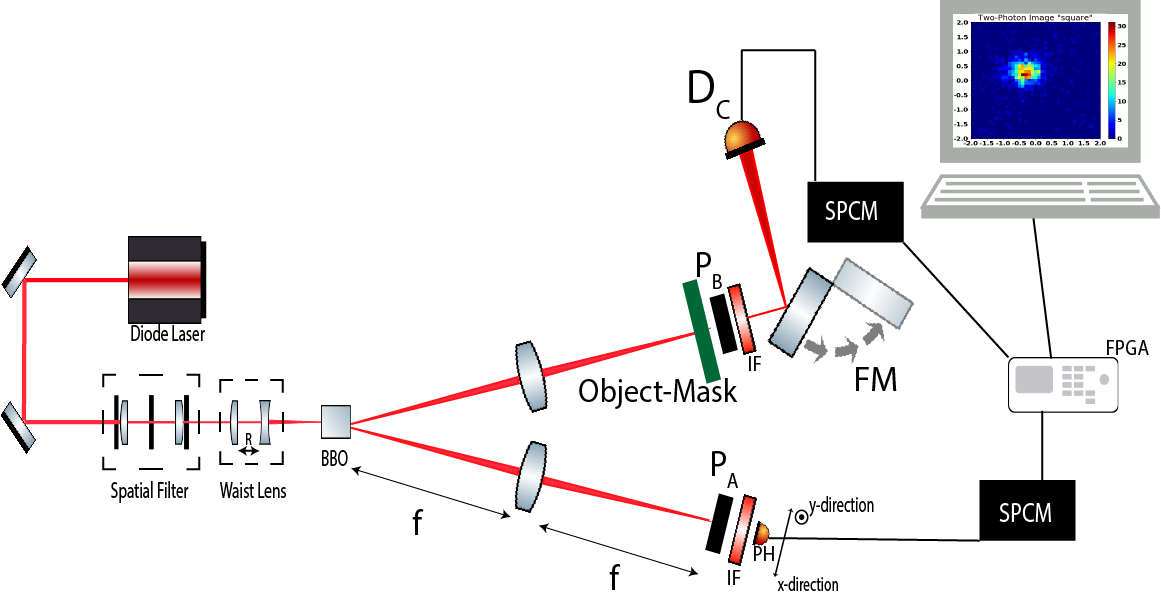
\includegraphics[width=1\textwidth]{Figures/ghostSetup2.png}
\caption{Experimental Setup for the Two-photon Imaging} 
\label{fig:ghostSetup}
\end{figure}

\subsection{Object-Mask}
This is an obstruction that is placed in the \textit{B} path. This is the object
from which we will make an image. It consist in an aperture on a translational mount,
that allow us to move the aperture precisely in the same plane we make our detections.
This is done by manipulating a pair of screws. 
We used differents objects and in Figure \ref{fig:mask1}
there is a detailed schematic of the first one used. It consists in a square aperture placed in the 4th 
quadrant of the scanned plane.

\begin{figure}[h!]
\centering
 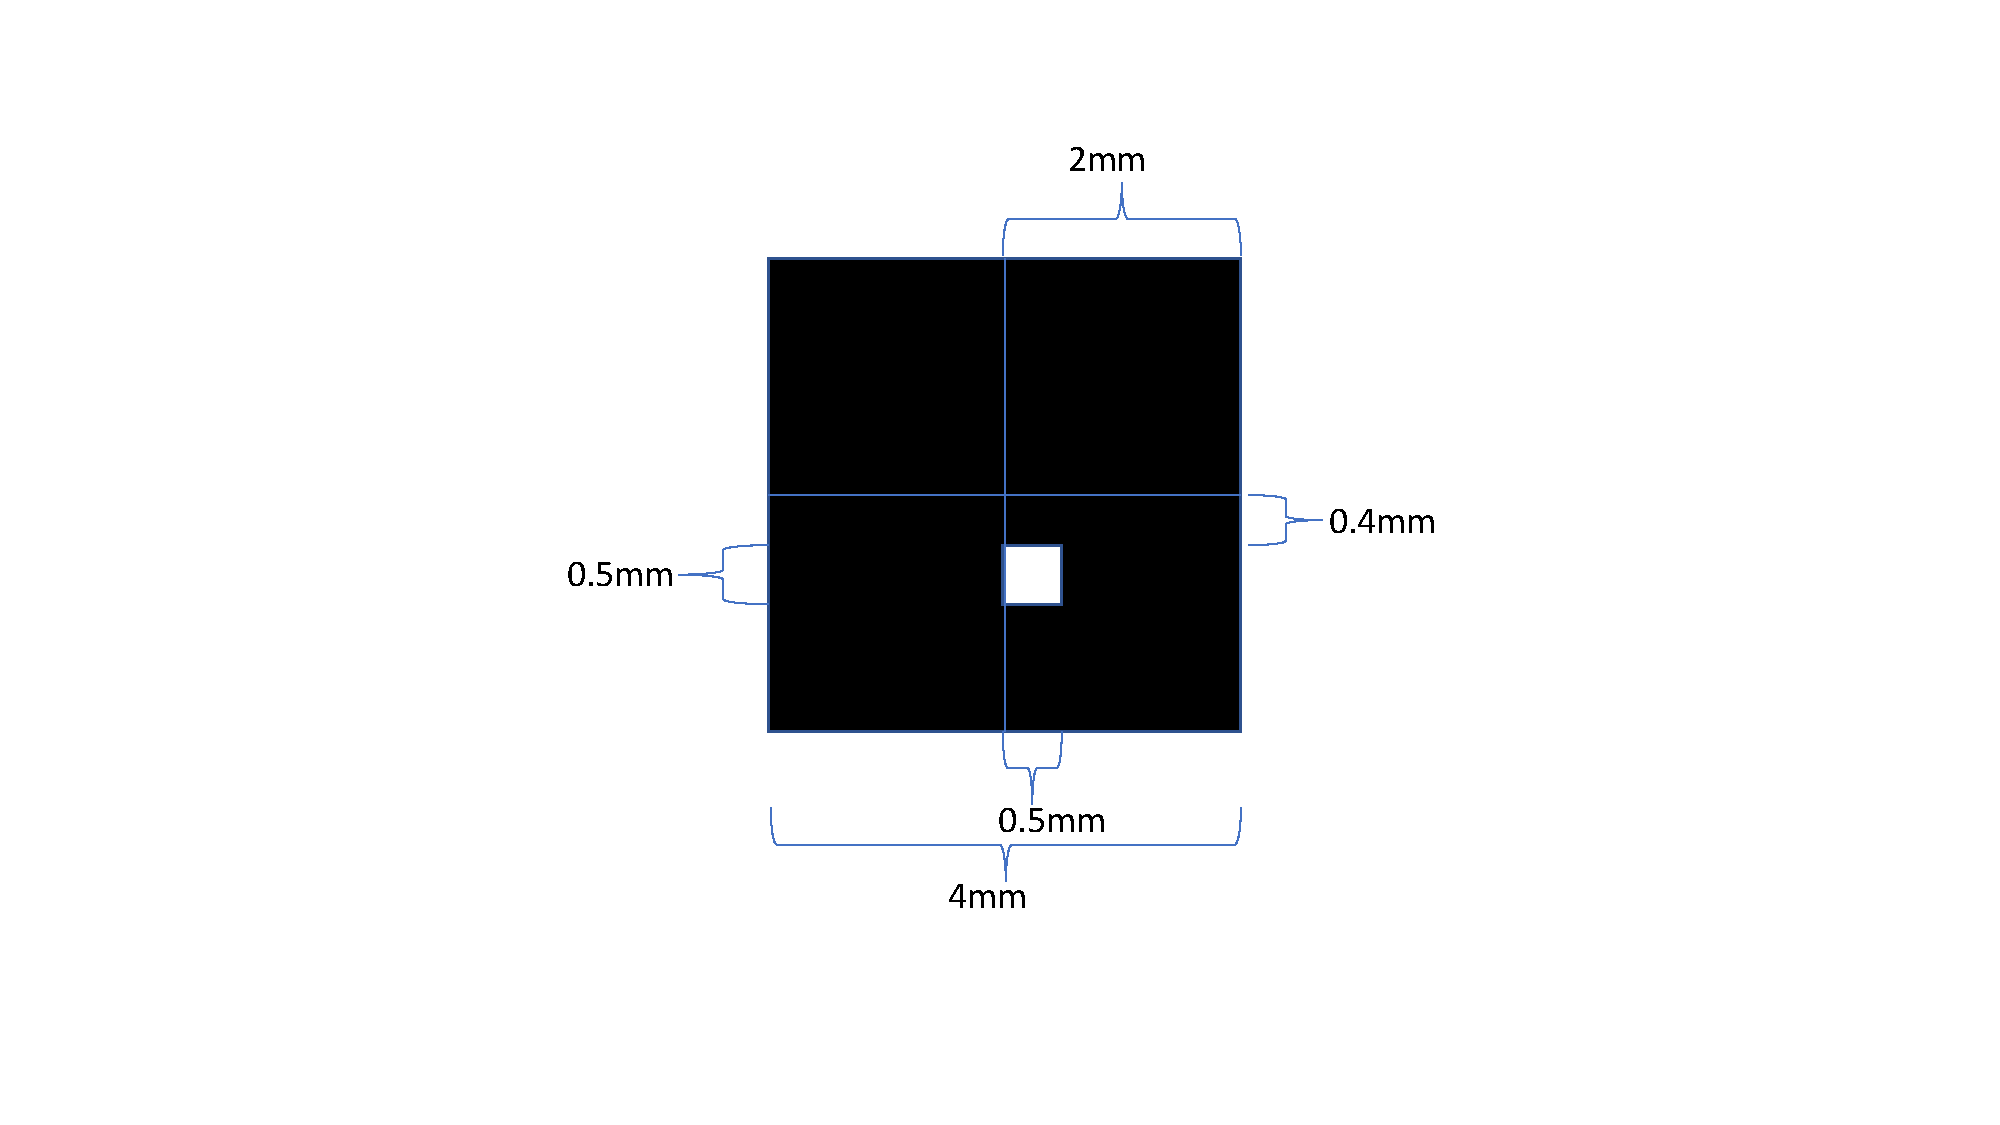
\includegraphics[width=0.6\textwidth]{Figures/mask1.pdf}
 \caption{Detailed description of the "square" aperture location in the scanned plane}
\label{fig:mask1} 
\end{figure}

In Figure \ref{fig:masks} there are the other two apertures that we used so far in the experiment, 
this apertures where selected because of the symmetries and antisymmetries they present, 
the goal of this monograh is to study the effect of the spatial correlations in the image
recovered, effect such as reflection of the original image, quality and others.  

\begin{figure}[h!]
\centering
{  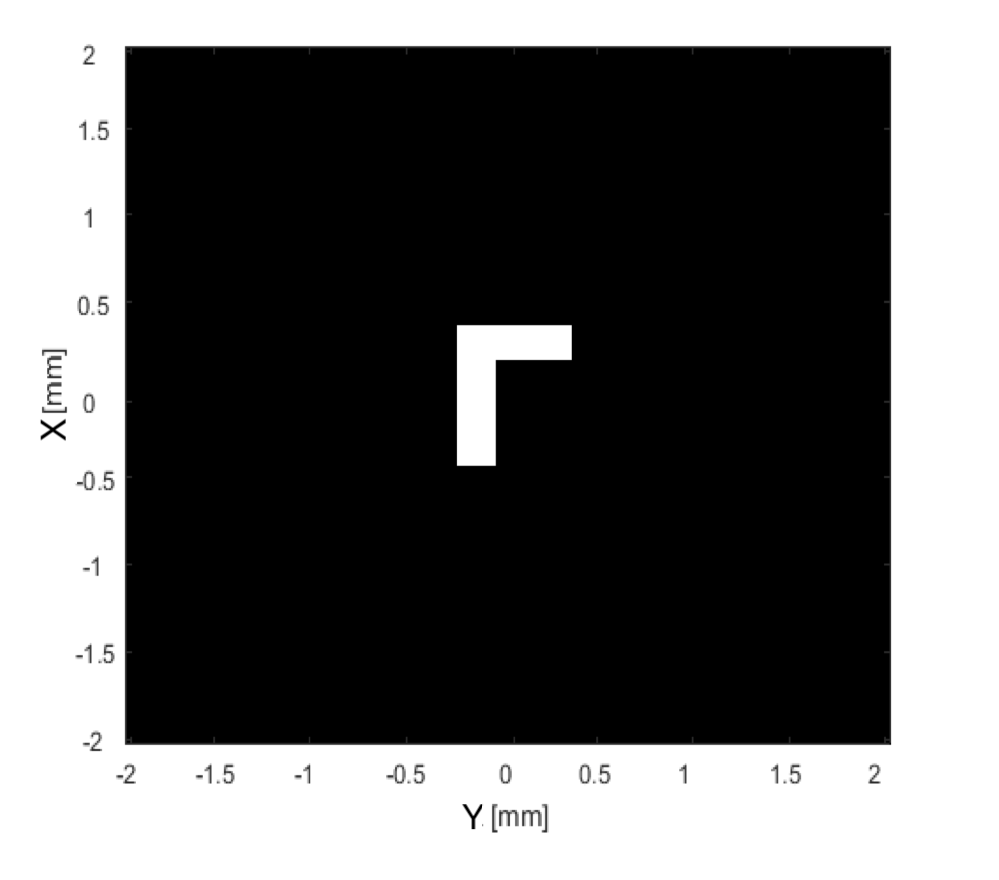
\includegraphics[width=0.45\textwidth]{Figures/mask2.png} }
{  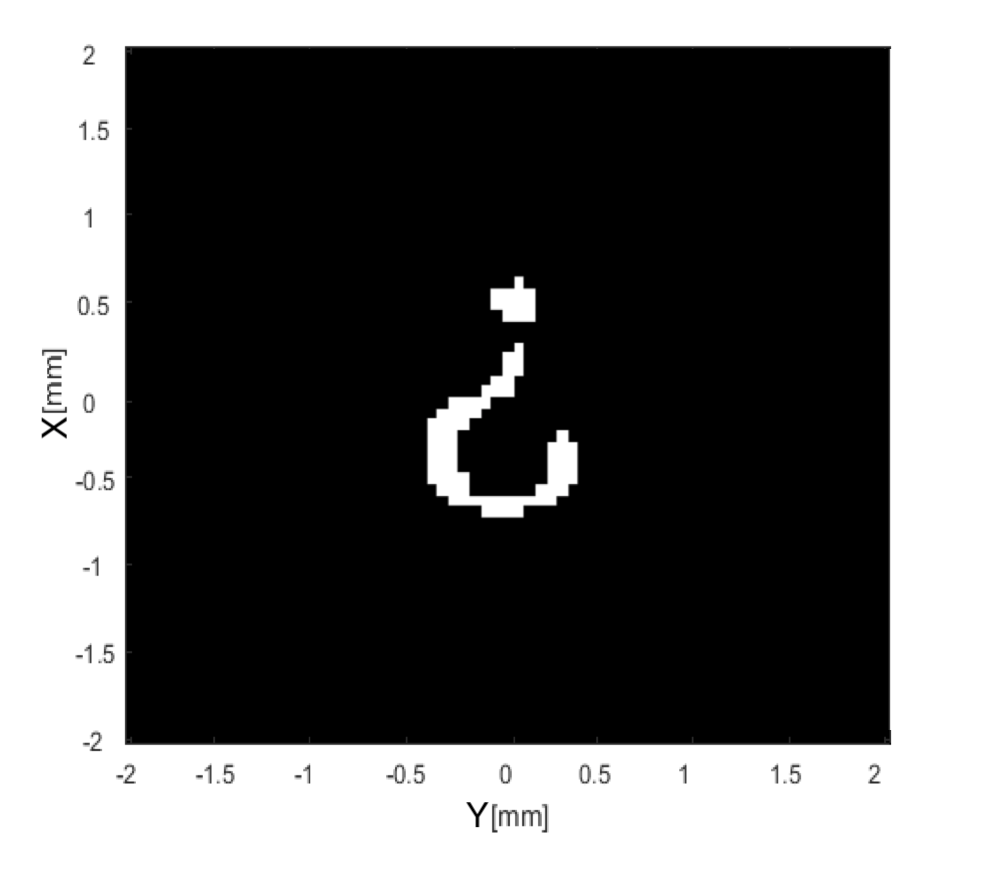
\includegraphics[width=0.45\textwidth]{Figures/mask3.png} }
\caption{The other two apertures used}
 \label{fig:masks}
\end{figure}

\subsection{Folding Mirror}
In order to change de path followed by the B-photon, and guide the light to a new detector $D_C$we use a Folding mirror, Figure \ref{fig:foldingMirror}.
This mirror plays the role of a switch, when is up, we are know dealing with the
$D_C$ detector, and we are doing a Two-photon Imaging process. In contrast, when the mirror is 
down, we are recovering spatial information, so it is possible to recognise some sort of
shadow from the object, or we are measuring the spatial correlations.
\begin{figure}[h!]
\centering
 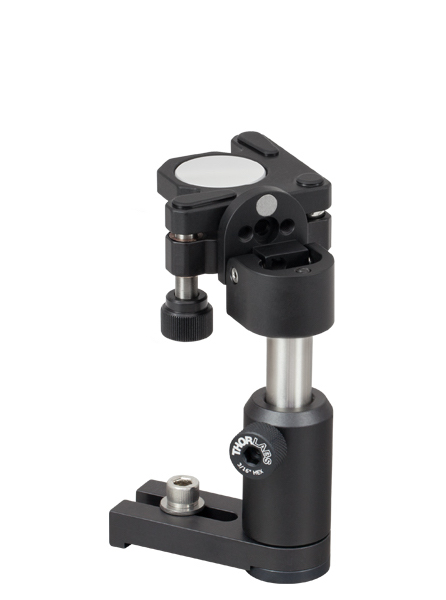
\includegraphics[width=0.25\textwidth]{Figures/foldingMirror.jpg}
 \caption{Foldind Mirror, it is in the position for measuring the correlations}
\label{fig:foldingMirror} 
\end{figure}

\subsection{Bucket Detector}
This detector consist denominated $D_C$ detector. It is a coupling lens that collects all the light that goes through the object.
The lens position is fixed, and it gathers all light and send it to a multi mode optical fiber connected to a SPCM.
In contrast to the other detections made before, the Bucket detector loses track of any spatial information of the photons. 
% Chapter Template

\chapter{Results} % Main chapter title

\label{Chapter4} % Change X to a consecutive number; for referencing this chapter elsewhere, use \ref{ChapterX}

%----------------------------------------------------------------------------------------
%	SECTION 1
%----------------------------------------------------------------------------------------
\section{Achiving a Gaussian Beam}

here comes de data od the new laser 

\section{Finding The Correlated Photons}

SPDC nocolinear type II
\begin{figure}[h!]
\centering
{  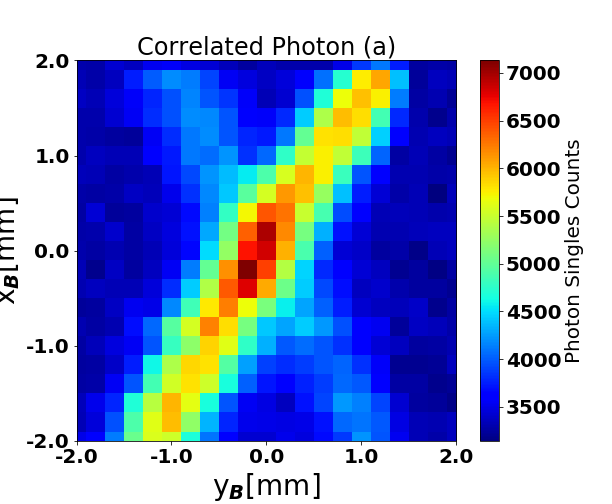
\includegraphics[width=0.45\textwidth]{Figures/correlatedPhotonSpot1.png} }
{  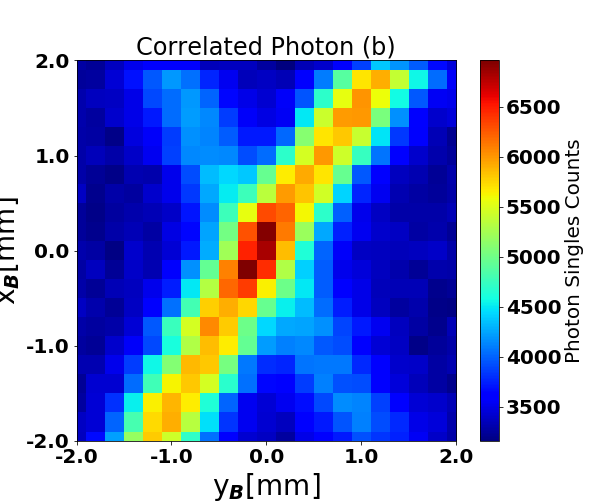
\includegraphics[width=0.45\textwidth]{Figures/correlatedPhotonSpot2.png} }
\caption{We are moving the translational translational stage, to locate the spot where the correlated photon are, for this try me moved the $y$ direction}
 \label{fig:correlatedPhotonSpot}
\end{figure}


\section{Experimental Correlations }

Info taken before me 
%-----------------------------------
%	SUBSECTION 1
%-----------------------------------
\subsection{$w_p = ?$}

\section{Mask Alignment}
We want that most of the correlated photon hits the mask 

\begin{figure}[h!]
\centering
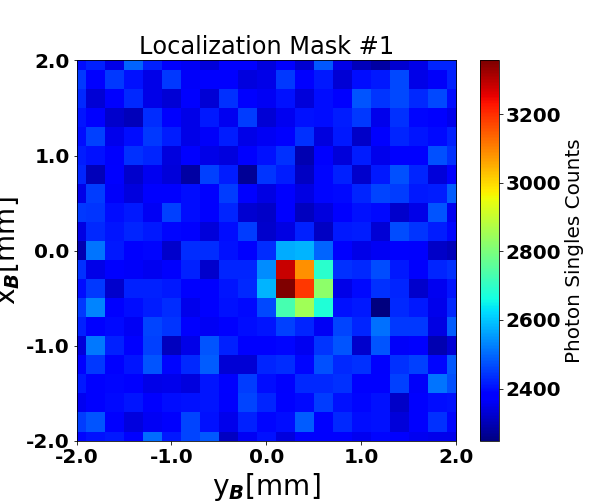
\includegraphics[width=0.6\textwidth]{Figures/localizationSq.png} 
\caption{Localization of the mask with an square}
\label{fig:localizationSq}
\end{figure}

changing to the mask with an L

\begin{figure}[h!]
\centering
{  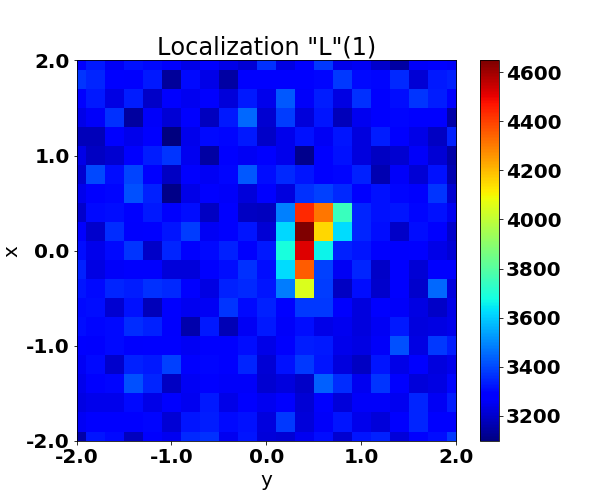
\includegraphics[width=0.45\textwidth]{Figures/localizationL1.png} }
{  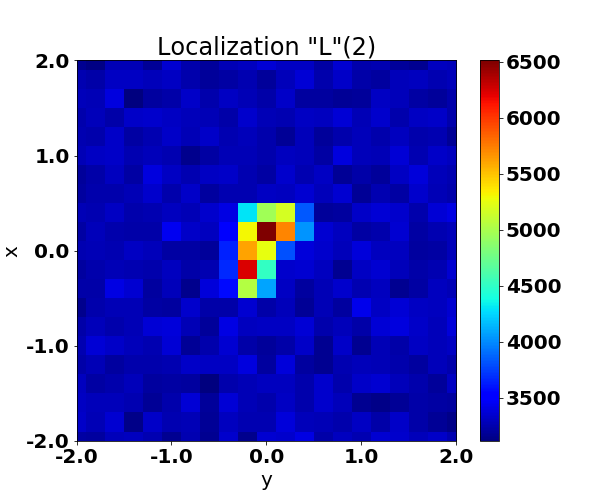
\includegraphics[width=0.45\textwidth]{Figures/localizationL2.png} }
\caption{Moving the L Mask in order to put it in the most central spot}
 \label{fig:localizationL}
\end{figure}
Long Exposure
\begin{figure}[h!]
\centering
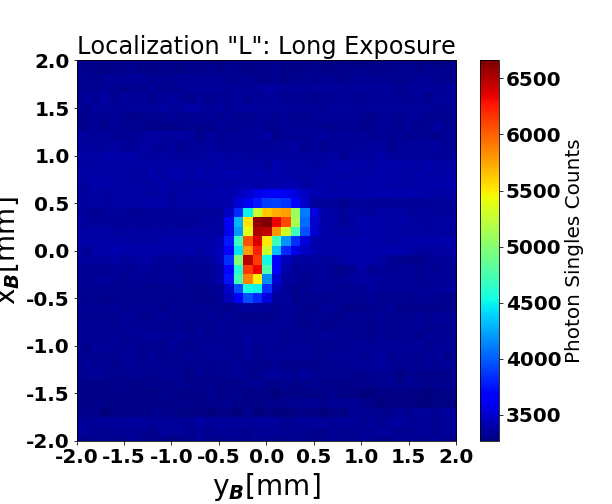
\includegraphics[width=0.6\textwidth]{Figures/localizationLLong.png} 
\caption{Long exposure of the definitive localization of the mask, in this try we leave the 
detector in each place for 30 seconds, we also make the steps of the detector smaller, $0.1mm$}
\label{fig:localizationDef}
\end{figure}

\section{Two-Photon Images}


\subsection{mask1}
\begin{figure}[h!]
\centering
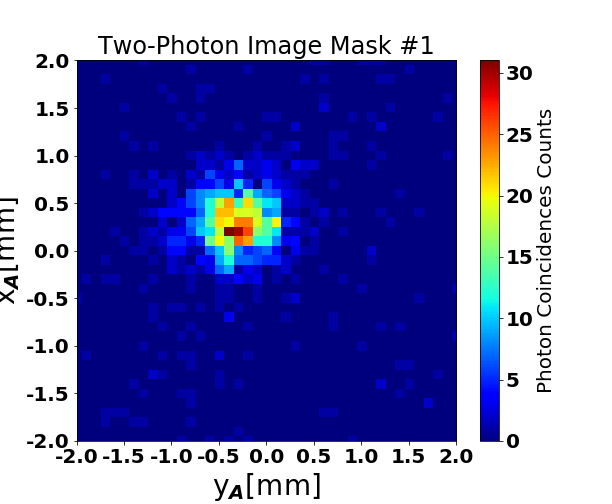
\includegraphics[width=0.6\textwidth]{Figures/two-photonImageSq.png} 
\caption{Localization of the mask with an square}
\label{fig:localizationSq}
\end{figure}

\subsection{mask2}
\subsection{mask3}
 
% Chapter Template

\chapter{Discussions and Conclusion} % Main chapter title

\label{Chapter5} % Change X to a consecutive number; for referencing this chapter elsewhere, use \ref{ChapterX}

%----------------------------------------------------------------------------------------
%	SECTION 1
%----------------------------------------------------------------------------------------


%% Chapter 1

\chapter{Chapter Title Here} % Main chapter title

\label{Chapter1} % For referencing the chapter elsewhere, use \ref{Chapter1} 

%----------------------------------------------------------------------------------------

% Define some commands to keep the formatting separated from the content 
\newcommand{\keyword}[1]{\textbf{#1}}
\newcommand{\tabhead}[1]{\textbf{#1}}
\newcommand{\code}[1]{\texttt{#1}}
\newcommand{\file}[1]{\texttt{\bfseries#1}}
\newcommand{\option}[1]{\texttt{\itshape#1}}

%----------------------------------------------------------------------------------------

\section{Welcome and Thank You}
Welcome to this \LaTeX{} Thesis Template, a beautiful and easy to use template for writing a thesis using the \LaTeX{} typesetting system.

If you are writing a thesis (or will be in the future) and its subject is technical or mathematical (though it doesn't have to be), then creating it in \LaTeX{} is highly recommended as a way to make sure you can just get down to the essential writing without having to worry over formatting or wasting time arguing with your word processor. 

\LaTeX{} is easily able to professionally typeset documents that run to hundreds or thousands of pages long. With simple mark-up commands, it automatically sets out the table of contents, margins, page headers and footers and keeps the formatting consistent and beautiful. One of its main strengths is the way it can easily typeset mathematics, even \emph{heavy} mathematics. Even if those equations are the most horribly twisted and most difficult mathematical problems that can only be solved on a super-computer, you can at least count on \LaTeX{} to make them look stunning.

%----------------------------------------------------------------------------------------

\section{Learning \LaTeX{}}

\LaTeX{} is not a \textsc{wysiwyg} (What You See is What You Get) program, unlike word processors such as Microsoft Word or Apple's Pages. Instead, a document written for \LaTeX{} is actually a simple, plain text file that contains \emph{no formatting}. You tell \LaTeX{} how you want the formatting in the finished document by writing in simple commands amongst the text, for example, if I want to use \emph{italic text for emphasis}, I write the \verb|\emph{text}| command and put the text I want in italics in between the curly braces. This means that \LaTeX{} is a \enquote{mark-up} language, very much like HTML.

\subsection{A (not so short) Introduction to \LaTeX{}}

If you are new to \LaTeX{}, there is a very good eBook -- freely available online as a PDF file -- called, \enquote{The Not So Short Introduction to \LaTeX{}}. The book's title is typically shortened to just \emph{lshort}. You can download the latest version (as it is occasionally updated) from here:
\url{http://www.ctan.org/tex-archive/info/lshort/english/lshort.pdf}

It is also available in several other languages. Find yours from the list on this page: \url{http://www.ctan.org/tex-archive/info/lshort/}

It is recommended to take a little time out to learn how to use \LaTeX{} by creating several, small `test' documents, or having a close look at several templates on:\\ 
\url{http://www.LaTeXTemplates.com}\\ 
Making the effort now means you're not stuck learning the system when what you \emph{really} need to be doing is writing your thesis.

\subsection{A Short Math Guide for \LaTeX{}}

If you are writing a technical or mathematical thesis, then you may want to read the document by the AMS (American Mathematical Society) called, \enquote{A Short Math Guide for \LaTeX{}}. It can be found online here:
\url{http://www.ams.org/tex/amslatex.html}
under the \enquote{Additional Documentation} section towards the bottom of the page.

\subsection{Common \LaTeX{} Math Symbols}
There are a multitude of mathematical symbols available for \LaTeX{} and it would take a great effort to learn the commands for them all. The most common ones you are likely to use are shown on this page:
\url{http://www.sunilpatel.co.uk/latex-type/latex-math-symbols/}

You can use this page as a reference or crib sheet, the symbols are rendered as large, high quality images so you can quickly find the \LaTeX{} command for the symbol you need.

\subsection{\LaTeX{} on a Mac}
 
The \LaTeX{} distribution is available for many systems including Windows, Linux and Mac OS X. The package for OS X is called MacTeX and it contains all the applications you need -- bundled together and pre-customized -- for a fully working \LaTeX{} environment and work flow.
 
MacTeX includes a custom dedicated \LaTeX{} editor called TeXShop for writing your `\file{.tex}' files and BibDesk: a program to manage your references and create your bibliography section just as easily as managing songs and creating playlists in iTunes.

%----------------------------------------------------------------------------------------

\section{Getting Started with this Template}

If you are familiar with \LaTeX{}, then you should explore the directory structure of the template and then proceed to place your own information into the \emph{THESIS INFORMATION} block of the \file{main.tex} file. You can then modify the rest of this file to your unique specifications based on your degree/university. Section \ref{FillingFile} on page \pageref{FillingFile} will help you do this. Make sure you also read section \ref{ThesisConventions} about thesis conventions to get the most out of this template.

If you are new to \LaTeX{} it is recommended that you carry on reading through the rest of the information in this document.

Before you begin using this template you should ensure that its style complies with the thesis style guidelines imposed by your institution. In most cases this template style and layout will be suitable. If it is not, it may only require a small change to bring the template in line with your institution's recommendations. These modifications will need to be done on the \file{MastersDoctoralThesis.cls} file.

\subsection{About this Template}

This \LaTeX{} Thesis Template is originally based and created around a \LaTeX{} style file created by Steve R.\ Gunn from the University of Southampton (UK), department of Electronics and Computer Science. You can find his original thesis style file at his site, here:
\url{http://www.ecs.soton.ac.uk/~srg/softwaretools/document/templates/}

Steve's \file{ecsthesis.cls} was then taken by Sunil Patel who modified it by creating a skeleton framework and folder structure to place the thesis files in. The resulting template can be found on Sunil's site here:
\url{http://www.sunilpatel.co.uk/thesis-template}

Sunil's template was made available through \url{http://www.LaTeXTemplates.com} where it was modified many times based on user requests and questions. Version 2.0 and onwards of this template represents a major modification to Sunil's template and is, in fact, hardly recognisable. The work to make version 2.0 possible was carried out by \href{mailto:vel@latextemplates.com}{Vel} and Johannes Böttcher.

%----------------------------------------------------------------------------------------

\section{What this Template Includes}

\subsection{Folders}

This template comes as a single zip file that expands out to several files and folders. The folder names are mostly self-explanatory:

\keyword{Appendices} -- this is the folder where you put the appendices. Each appendix should go into its own separate \file{.tex} file. An example and template are included in the directory.

\keyword{Chapters} -- this is the folder where you put the thesis chapters. A thesis usually has about six chapters, though there is no hard rule on this. Each chapter should go in its own separate \file{.tex} file and they can be split as:
\begin{itemize}
\item Chapter 1: Introduction to the thesis topic
\item Chapter 2: Background information and theory
\item Chapter 3: (Laboratory) experimental setup
\item Chapter 4: Details of experiment 1
\item Chapter 5: Details of experiment 2
\item Chapter 6: Discussion of the experimental results
\item Chapter 7: Conclusion and future directions
\end{itemize}
This chapter layout is specialised for the experimental sciences, your discipline may be different.

\keyword{Figures} -- this folder contains all figures for the thesis. These are the final images that will go into the thesis document.

\subsection{Files}

Included are also several files, most of them are plain text and you can see their contents in a text editor. After initial compilation, you will see that more auxiliary files are created by \LaTeX{} or BibTeX and which you don't need to delete or worry about:

\keyword{example.bib} -- this is an important file that contains all the bibliographic information and references that you will be citing in the thesis for use with BibTeX. You can write it manually, but there are reference manager programs available that will create and manage it for you. Bibliographies in \LaTeX{} are a large subject and you may need to read about BibTeX before starting with this. Many modern reference managers will allow you to export your references in BibTeX format which greatly eases the amount of work you have to do.

\keyword{MastersDoctoralThesis.cls} -- this is an important file. It is the class file that tells \LaTeX{} how to format the thesis. 

\keyword{main.pdf} -- this is your beautifully typeset thesis (in the PDF file format) created by \LaTeX{}. It is supplied in the PDF with the template and after you compile the template you should get an identical version.

\keyword{main.tex} -- this is an important file. This is the file that you tell \LaTeX{} to compile to produce your thesis as a PDF file. It contains the framework and constructs that tell \LaTeX{} how to layout the thesis. It is heavily commented so you can read exactly what each line of code does and why it is there. After you put your own information into the \emph{THESIS INFORMATION} block -- you have now started your thesis!

Files that are \emph{not} included, but are created by \LaTeX{} as auxiliary files include:

\keyword{main.aux} -- this is an auxiliary file generated by \LaTeX{}, if it is deleted \LaTeX{} simply regenerates it when you run the main \file{.tex} file.

\keyword{main.bbl} -- this is an auxiliary file generated by BibTeX, if it is deleted, BibTeX simply regenerates it when you run the \file{main.aux} file. Whereas the \file{.bib} file contains all the references you have, this \file{.bbl} file contains the references you have actually cited in the thesis and is used to build the bibliography section of the thesis.

\keyword{main.blg} -- this is an auxiliary file generated by BibTeX, if it is deleted BibTeX simply regenerates it when you run the main \file{.aux} file.

\keyword{main.lof} -- this is an auxiliary file generated by \LaTeX{}, if it is deleted \LaTeX{} simply regenerates it when you run the main \file{.tex} file. It tells \LaTeX{} how to build the \emph{List of Figures} section.

\keyword{main.log} -- this is an auxiliary file generated by \LaTeX{}, if it is deleted \LaTeX{} simply regenerates it when you run the main \file{.tex} file. It contains messages from \LaTeX{}, if you receive errors and warnings from \LaTeX{}, they will be in this \file{.log} file.

\keyword{main.lot} -- this is an auxiliary file generated by \LaTeX{}, if it is deleted \LaTeX{} simply regenerates it when you run the main \file{.tex} file. It tells \LaTeX{} how to build the \emph{List of Tables} section.

\keyword{main.out} -- this is an auxiliary file generated by \LaTeX{}, if it is deleted \LaTeX{} simply regenerates it when you run the main \file{.tex} file.

So from this long list, only the files with the \file{.bib}, \file{.cls} and \file{.tex} extensions are the most important ones. The other auxiliary files can be ignored or deleted as \LaTeX{} and BibTeX will regenerate them.

%----------------------------------------------------------------------------------------

\section{Filling in Your Information in the \file{main.tex} File}\label{FillingFile}

You will need to personalise the thesis template and make it your own by filling in your own information. This is done by editing the \file{main.tex} file in a text editor or your favourite LaTeX environment.

Open the file and scroll down to the third large block titled \emph{THESIS INFORMATION} where you can see the entries for \emph{University Name}, \emph{Department Name}, etc \ldots

Fill out the information about yourself, your group and institution. You can also insert web links, if you do, make sure you use the full URL, including the \code{http://} for this. If you don't want these to be linked, simply remove the \verb|\href{url}{name}| and only leave the name.

When you have done this, save the file and recompile \code{main.tex}. All the information you filled in should now be in the PDF, complete with web links. You can now begin your thesis proper!

%----------------------------------------------------------------------------------------

\section{The \code{main.tex} File Explained}

The \file{main.tex} file contains the structure of the thesis. There are plenty of written comments that explain what pages, sections and formatting the \LaTeX{} code is creating. Each major document element is divided into commented blocks with titles in all capitals to make it obvious what the following bit of code is doing. Initially there seems to be a lot of \LaTeX{} code, but this is all formatting, and it has all been taken care of so you don't have to do it.

Begin by checking that your information on the title page is correct. For the thesis declaration, your institution may insist on something different than the text given. If this is the case, just replace what you see with what is required in the \emph{DECLARATION PAGE} block.

Then comes a page which contains a funny quote. You can put your own, or quote your favourite scientist, author, person, and so on. Make sure to put the name of the person who you took the quote from.

Following this is the abstract page which summarises your work in a condensed way and can almost be used as a standalone document to describe what you have done. The text you write will cause the heading to move up so don't worry about running out of space.

Next come the acknowledgements. On this page, write about all the people who you wish to thank (not forgetting parents, partners and your advisor/supervisor).

The contents pages, list of figures and tables are all taken care of for you and do not need to be manually created or edited. The next set of pages are more likely to be optional and can be deleted since they are for a more technical thesis: insert a list of abbreviations you have used in the thesis, then a list of the physical constants and numbers you refer to and finally, a list of mathematical symbols used in any formulae. Making the effort to fill these tables means the reader has a one-stop place to refer to instead of searching the internet and references to try and find out what you meant by certain abbreviations or symbols.

The list of symbols is split into the Roman and Greek alphabets. Whereas the abbreviations and symbols ought to be listed in alphabetical order (and this is \emph{not} done automatically for you) the list of physical constants should be grouped into similar themes.

The next page contains a one line dedication. Who will you dedicate your thesis to?

Finally, there is the block where the chapters are included. Uncomment the lines (delete the \code{\%} character) as you write the chapters. Each chapter should be written in its own file and put into the \emph{Chapters} folder and named \file{Chapter1}, \file{Chapter2}, etc\ldots Similarly for the appendices, uncomment the lines as you need them. Each appendix should go into its own file and placed in the \emph{Appendices} folder.

After the preamble, chapters and appendices finally comes the bibliography. The bibliography style (called \option{authoryear}) is used for the bibliography and is a fully featured style that will even include links to where the referenced paper can be found online. Do not underestimate how grateful your reader will be to find that a reference to a paper is just a click away. Of course, this relies on you putting the URL information into the BibTeX file in the first place.

%----------------------------------------------------------------------------------------

\section{Thesis Features and Conventions}\label{ThesisConventions}

To get the best out of this template, there are a few conventions that you may want to follow.

One of the most important (and most difficult) things to keep track of in such a long document as a thesis is consistency. Using certain conventions and ways of doing things (such as using a Todo list) makes the job easier. Of course, all of these are optional and you can adopt your own method.

\subsection{Printing Format}

This thesis template is designed for double sided printing (i.e. content on the front and back of pages) as most theses are printed and bound this way. Switching to one sided printing is as simple as uncommenting the \option{oneside} option of the \code{documentclass} command at the top of the \file{main.tex} file. You may then wish to adjust the margins to suit specifications from your institution.

The headers for the pages contain the page number on the outer side (so it is easy to flick through to the page you want) and the chapter name on the inner side.

The text is set to 11 point by default with single line spacing, again, you can tune the text size and spacing should you want or need to using the options at the very start of \file{main.tex}. The spacing can be changed similarly by replacing the \option{singlespacing} with \option{onehalfspacing} or \option{doublespacing}.

\subsection{Using US Letter Paper}

The paper size used in the template is A4, which is the standard size in Europe. If you are using this thesis template elsewhere and particularly in the United States, then you may have to change the A4 paper size to the US Letter size. This can be done in the margins settings section in \file{main.tex}.

Due to the differences in the paper size, the resulting margins may be different to what you like or require (as it is common for institutions to dictate certain margin sizes). If this is the case, then the margin sizes can be tweaked by modifying the values in the same block as where you set the paper size. Now your document should be set up for US Letter paper size with suitable margins.


\subsubsection{A Note on bibtex}

The bibtex backend used in the template by default does not correctly handle unicode character encoding (i.e. "international" characters). You may see a warning about this in the compilation log and, if your references contain unicode characters, they may not show up correctly or at all. The solution to this is to use the biber backend instead of the outdated bibtex backend. This is done by finding this in \file{main.tex}: \option{backend=bibtex} and changing it to \option{backend=biber}. You will then need to delete all auxiliary BibTeX files and navigate to the template directory in your terminal (command prompt). Once there, simply type \code{biber main} and biber will compile your bibliography. You can then compile \file{main.tex} as normal and your bibliography will be updated. An alternative is to set up your LaTeX editor to compile with biber instead of bibtex, see \href{http://tex.stackexchange.com/questions/154751/biblatex-with-biber-configuring-my-editor-to-avoid-undefined-citations/}{here} for how to do this for various editors.

\subsection{Tables}

Tables are an important way of displaying your results, below is an example table which was generated with this code:

{\small
\begin{verbatim}
\begin{table}
\caption{The effects of treatments X and Y on the four groups studied.}
\label{tab:treatments}
\centering
\begin{tabular}{l l l}
\toprule
\tabhead{Groups} & \tabhead{Treatment X} & \tabhead{Treatment Y} \\
\midrule
1 & 0.2 & 0.8\\
2 & 0.17 & 0.7\\
3 & 0.24 & 0.75\\
4 & 0.68 & 0.3\\
\bottomrule\\
\end{tabular}
\end{table}
\end{verbatim}
}

\begin{table}
\caption{The effects of treatments X and Y on the four groups studied.}
\label{tab:treatments}
\centering
\begin{tabular}{l l l}
\toprule
\tabhead{Groups} & \tabhead{Treatment X} & \tabhead{Treatment Y} \\
\midrule
1 & 0.2 & 0.8\\
2 & 0.17 & 0.7\\
3 & 0.24 & 0.75\\
4 & 0.68 & 0.3\\
\bottomrule\\
\end{tabular}
\end{table}

You can reference tables with \verb|\ref{<label>}| where the label is defined within the table environment. See \file{Chapter1.tex} for an example of the label and citation (e.g. Table~\ref{tab:treatments}).

\subsection{Figures}

There will hopefully be many figures in your thesis (that should be placed in the \emph{Figures} folder). The way to insert figures into your thesis is to use a code template like this:
\begin{verbatim}
\begin{figure}
\centering

\includegraphics{Figures/Electron}
\decoRule
\caption[An Electron]{An electron (artist's impression).}
\label{fig:Electron}
\end{figure}
\end{verbatim}
Also look in the source file. Putting this code into the source file produces the picture of the electron that you can see in the figure below.

\begin{figure}[th]
\centering

\includegraphics{Figures/Electron}
\decoRule
\caption[An Electron]{An electron (artist's impression).}
\label{fig:Electron}
\end{figure}

Sometimes figures don't always appear where you write them in the source. The placement depends on how much space there is on the page for the figure. Sometimes there is not enough room to fit a figure directly where it should go (in relation to the text) and so \LaTeX{} puts it at the top of the next page. Positioning figures is the job of \LaTeX{} and so you should only worry about making them look good!

Figures usually should have captions just in case you need to refer to them (such as in Figure~\ref{fig:Electron}). The \verb|\caption| command contains two parts, the first part, inside the square brackets is the title that will appear in the \emph{List of Figures}, and so should be short. The second part in the curly brackets should contain the longer and more descriptive caption text.

The \verb|\decoRule| command is optional and simply puts an aesthetic horizontal line below the image. If you do this for one image, do it for all of them.

\LaTeX{} is capable of using images in pdf, jpg and png format.

\subsection{Typesetting mathematics}

If your thesis is going to contain heavy mathematical content, be sure that \LaTeX{} will make it look beautiful, even though it won't be able to solve the equations for you.

The \enquote{Not So Short Introduction to \LaTeX} (available on \href{http://www.ctan.org/tex-archive/info/lshort/english/lshort.pdf}{CTAN}) should tell you everything you need to know for most cases of typesetting mathematics. If you need more information, a much more thorough mathematical guide is available from the AMS called, \enquote{A Short Math Guide to \LaTeX} and can be downloaded from:
\url{ftp://ftp.ams.org/pub/tex/doc/amsmath/short-math-guide.pdf}

There are many different \LaTeX{} symbols to remember, luckily you can find the most common symbols in \href{http://ctan.org/pkg/comprehensive}{The Comprehensive \LaTeX~Symbol List}.

You can write an equation, which is automatically given an equation number by \LaTeX{} like this:
\begin{verbatim}
\begin{equation}
E = mc^{2}
\label{eqn:Einstein}
\end{equation}
\end{verbatim}

This will produce Einstein's famous energy-matter equivalence equation:
\begin{equation}
E = mc^{2}
\label{eqn:Einstein}
\end{equation}

All equations you write (which are not in the middle of paragraph text) are automatically given equation numbers by \LaTeX{}. If you don't want a particular equation numbered, use the unnumbered form:
\begin{verbatim}
\[ a^{2}=4 \]
\end{verbatim}

%----------------------------------------------------------------------------------------

\section{Sectioning and Subsectioning}

You should break your thesis up into nice, bite-sized sections and subsections. \LaTeX{} automatically builds a table of Contents by looking at all the \verb|\chapter{}|, \verb|\section{}|  and \verb|\subsection{}| commands you write in the source.

The Table of Contents should only list the sections to three (3) levels. A \verb|chapter{}| is level zero (0). A \verb|\section{}| is level one (1) and so a \verb|\subsection{}| is level two (2). In your thesis it is likely that you will even use a \verb|subsubsection{}|, which is level three (3). The depth to which the Table of Contents is formatted is set within \file{MastersDoctoralThesis.cls}. If you need this changed, you can do it in \file{main.tex}.

%----------------------------------------------------------------------------------------

\section{In Closing}

You have reached the end of this mini-guide. You can now rename or overwrite this pdf file and begin writing your own \file{Chapter1.tex} and the rest of your thesis. The easy work of setting up the structure and framework has been taken care of for you. It's now your job to fill it out!

Good luck and have lots of fun!

\begin{flushright}
Guide written by ---\\
Sunil Patel: \href{http://www.sunilpatel.co.uk}{www.sunilpatel.co.uk}\\
Vel: \href{http://www.LaTeXTemplates.com}{LaTeXTemplates.com}
\end{flushright}
 

%----------------------------------------------------------------------------------------
%	THESIS CONTENT - APPENDICES
%----------------------------------------------------------------------------------------

\appendix % Cue to tell LaTeX that the following "chapters" are Appendices

% Include the appendices of the thesis as separate files from the Appendices folder
% Uncomment the lines as you write the Appendices

%% Appendix A

\chapter{Intensity at the Image Plane} % Main appendix title

\label{app:intensity} % For referencing this appendix elsewhere, use \ref{AppendixA}

\section{How do I change the colors of links?}

The color of links can be changed to your liking using:

{\small\verb!\hypersetup{urlcolor=red}!}, or

{\small\verb!\hypersetup{citecolor=green}!}, or

{\small\verb!\hypersetup{allcolor=blue}!}.

\noindent If you want to completely hide the links, you can use:

{\small\verb!\hypersetup{allcolors=.}!}, or even better: 

{\small\verb!\hypersetup{hidelinks}!}.

\noindent If you want to have obvious links in the PDF but not the printed text, use:

{\small\verb!\hypersetup{colorlinks=false}!}.

%\include{Appendices/AppendixB}
%\include{Appendices/AppendixC}

%----------------------------------------------------------------------------------------
%	BIBLIOGRAPHY
%----------------------------------------------------------------------------------------

\bibliography{Bibliography}
\bibliographystyle{unsrt}
%\bibliographystyle{siam}

%\printbibliography
%\printbibliography[heading=bibintoc]

%----------------------------------------------------------------------------------------

\end{document}  
